% Options for packages loaded elsewhere
\PassOptionsToPackage{unicode}{hyperref}
\PassOptionsToPackage{hyphens}{url}
%
\documentclass[
]{book}
\title{Data Visualisation \texttt{geom} Encyclopedia}
\author{Thiyanga S. Talagala}
\date{2023-08-31}

\usepackage{amsmath,amssymb}
\usepackage{lmodern}
\usepackage{iftex}
\ifPDFTeX
  \usepackage[T1]{fontenc}
  \usepackage[utf8]{inputenc}
  \usepackage{textcomp} % provide euro and other symbols
\else % if luatex or xetex
  \usepackage{unicode-math}
  \defaultfontfeatures{Scale=MatchLowercase}
  \defaultfontfeatures[\rmfamily]{Ligatures=TeX,Scale=1}
\fi
% Use upquote if available, for straight quotes in verbatim environments
\IfFileExists{upquote.sty}{\usepackage{upquote}}{}
\IfFileExists{microtype.sty}{% use microtype if available
  \usepackage[]{microtype}
  \UseMicrotypeSet[protrusion]{basicmath} % disable protrusion for tt fonts
}{}
\makeatletter
\@ifundefined{KOMAClassName}{% if non-KOMA class
  \IfFileExists{parskip.sty}{%
    \usepackage{parskip}
  }{% else
    \setlength{\parindent}{0pt}
    \setlength{\parskip}{6pt plus 2pt minus 1pt}}
}{% if KOMA class
  \KOMAoptions{parskip=half}}
\makeatother
\usepackage{xcolor}
\IfFileExists{xurl.sty}{\usepackage{xurl}}{} % add URL line breaks if available
\IfFileExists{bookmark.sty}{\usepackage{bookmark}}{\usepackage{hyperref}}
\hypersetup{
  pdftitle={Data Visualisation geom Encyclopedia},
  pdfauthor={Thiyanga S. Talagala},
  hidelinks,
  pdfcreator={LaTeX via pandoc}}
\urlstyle{same} % disable monospaced font for URLs
\usepackage{color}
\usepackage{fancyvrb}
\newcommand{\VerbBar}{|}
\newcommand{\VERB}{\Verb[commandchars=\\\{\}]}
\DefineVerbatimEnvironment{Highlighting}{Verbatim}{commandchars=\\\{\}}
% Add ',fontsize=\small' for more characters per line
\usepackage{framed}
\definecolor{shadecolor}{RGB}{248,248,248}
\newenvironment{Shaded}{\begin{snugshade}}{\end{snugshade}}
\newcommand{\AlertTok}[1]{\textcolor[rgb]{0.94,0.16,0.16}{#1}}
\newcommand{\AnnotationTok}[1]{\textcolor[rgb]{0.56,0.35,0.01}{\textbf{\textit{#1}}}}
\newcommand{\AttributeTok}[1]{\textcolor[rgb]{0.77,0.63,0.00}{#1}}
\newcommand{\BaseNTok}[1]{\textcolor[rgb]{0.00,0.00,0.81}{#1}}
\newcommand{\BuiltInTok}[1]{#1}
\newcommand{\CharTok}[1]{\textcolor[rgb]{0.31,0.60,0.02}{#1}}
\newcommand{\CommentTok}[1]{\textcolor[rgb]{0.56,0.35,0.01}{\textit{#1}}}
\newcommand{\CommentVarTok}[1]{\textcolor[rgb]{0.56,0.35,0.01}{\textbf{\textit{#1}}}}
\newcommand{\ConstantTok}[1]{\textcolor[rgb]{0.00,0.00,0.00}{#1}}
\newcommand{\ControlFlowTok}[1]{\textcolor[rgb]{0.13,0.29,0.53}{\textbf{#1}}}
\newcommand{\DataTypeTok}[1]{\textcolor[rgb]{0.13,0.29,0.53}{#1}}
\newcommand{\DecValTok}[1]{\textcolor[rgb]{0.00,0.00,0.81}{#1}}
\newcommand{\DocumentationTok}[1]{\textcolor[rgb]{0.56,0.35,0.01}{\textbf{\textit{#1}}}}
\newcommand{\ErrorTok}[1]{\textcolor[rgb]{0.64,0.00,0.00}{\textbf{#1}}}
\newcommand{\ExtensionTok}[1]{#1}
\newcommand{\FloatTok}[1]{\textcolor[rgb]{0.00,0.00,0.81}{#1}}
\newcommand{\FunctionTok}[1]{\textcolor[rgb]{0.00,0.00,0.00}{#1}}
\newcommand{\ImportTok}[1]{#1}
\newcommand{\InformationTok}[1]{\textcolor[rgb]{0.56,0.35,0.01}{\textbf{\textit{#1}}}}
\newcommand{\KeywordTok}[1]{\textcolor[rgb]{0.13,0.29,0.53}{\textbf{#1}}}
\newcommand{\NormalTok}[1]{#1}
\newcommand{\OperatorTok}[1]{\textcolor[rgb]{0.81,0.36,0.00}{\textbf{#1}}}
\newcommand{\OtherTok}[1]{\textcolor[rgb]{0.56,0.35,0.01}{#1}}
\newcommand{\PreprocessorTok}[1]{\textcolor[rgb]{0.56,0.35,0.01}{\textit{#1}}}
\newcommand{\RegionMarkerTok}[1]{#1}
\newcommand{\SpecialCharTok}[1]{\textcolor[rgb]{0.00,0.00,0.00}{#1}}
\newcommand{\SpecialStringTok}[1]{\textcolor[rgb]{0.31,0.60,0.02}{#1}}
\newcommand{\StringTok}[1]{\textcolor[rgb]{0.31,0.60,0.02}{#1}}
\newcommand{\VariableTok}[1]{\textcolor[rgb]{0.00,0.00,0.00}{#1}}
\newcommand{\VerbatimStringTok}[1]{\textcolor[rgb]{0.31,0.60,0.02}{#1}}
\newcommand{\WarningTok}[1]{\textcolor[rgb]{0.56,0.35,0.01}{\textbf{\textit{#1}}}}
\usepackage{longtable,booktabs,array}
\usepackage{calc} % for calculating minipage widths
% Correct order of tables after \paragraph or \subparagraph
\usepackage{etoolbox}
\makeatletter
\patchcmd\longtable{\par}{\if@noskipsec\mbox{}\fi\par}{}{}
\makeatother
% Allow footnotes in longtable head/foot
\IfFileExists{footnotehyper.sty}{\usepackage{footnotehyper}}{\usepackage{footnote}}
\makesavenoteenv{longtable}
\usepackage{graphicx}
\makeatletter
\def\maxwidth{\ifdim\Gin@nat@width>\linewidth\linewidth\else\Gin@nat@width\fi}
\def\maxheight{\ifdim\Gin@nat@height>\textheight\textheight\else\Gin@nat@height\fi}
\makeatother
% Scale images if necessary, so that they will not overflow the page
% margins by default, and it is still possible to overwrite the defaults
% using explicit options in \includegraphics[width, height, ...]{}
\setkeys{Gin}{width=\maxwidth,height=\maxheight,keepaspectratio}
% Set default figure placement to htbp
\makeatletter
\def\fps@figure{htbp}
\makeatother
\setlength{\emergencystretch}{3em} % prevent overfull lines
\providecommand{\tightlist}{%
  \setlength{\itemsep}{0pt}\setlength{\parskip}{0pt}}
\setcounter{secnumdepth}{5}
\usepackage{booktabs}
\ifLuaTeX
  \usepackage{selnolig}  % disable illegal ligatures
\fi
\usepackage[]{biblatex}
\addbibresource{book.bib}
\addbibresource{packages.bib}

\begin{document}
\maketitle

{
\setcounter{tocdepth}{1}
\tableofcontents
}
\hypertarget{about}{%
\chapter{About}\label{about}}

This is a \emph{sample} book written in \textbf{Markdown}. You can use anything that Pandoc's Markdown supports; for example, a math equation \(a^2 + b^2 = c^2\).

\hypertarget{usage}{%
\section{Usage}\label{usage}}

Each \textbf{bookdown} chapter is an .Rmd file, and each .Rmd file can contain one (and only one) chapter. A chapter \emph{must} start with a first-level heading: \texttt{\#\ A\ good\ chapter}, and can contain one (and only one) first-level heading.

Use second-level and higher headings within chapters like: \texttt{\#\#\ A\ short\ section} or \texttt{\#\#\#\ An\ even\ shorter\ section}.

The \texttt{index.Rmd} file is required, and is also your first book chapter. It will be the homepage when you render the book.

\hypertarget{render-book}{%
\section{Render book}\label{render-book}}

You can render the HTML version of this example book without changing anything:

\begin{enumerate}
\def\labelenumi{\arabic{enumi}.}
\item
  Find the \textbf{Build} pane in the RStudio IDE, and
\item
  Click on \textbf{Build Book}, then select your output format, or select ``All formats'' if you'd like to use multiple formats from the same book source files.
\end{enumerate}

Or build the book from the R console:

\begin{Shaded}
\begin{Highlighting}[]
\NormalTok{bookdown}\SpecialCharTok{::}\FunctionTok{render\_book}\NormalTok{()}
\end{Highlighting}
\end{Shaded}

To render this example to PDF as a \texttt{bookdown::pdf\_book}, you'll need to install XeLaTeX. You are recommended to install TinyTeX (which includes XeLaTeX): \url{https://yihui.org/tinytex/}.

\hypertarget{preview-book}{%
\section{Preview book}\label{preview-book}}

As you work, you may start a local server to live preview this HTML book. This preview will update as you edit the book when you save individual .Rmd files. You can start the server in a work session by using the RStudio add-in ``Preview book'', or from the R console:

\begin{Shaded}
\begin{Highlighting}[]
\NormalTok{bookdown}\SpecialCharTok{::}\FunctionTok{serve\_book}\NormalTok{()}
\end{Highlighting}
\end{Shaded}

\hypertarget{hello-bookdown}{%
\chapter{Hello bookdown}\label{hello-bookdown}}

All chapters start with a first-level heading followed by your chapter title, like the line above. There should be only one first-level heading (\texttt{\#}) per .Rmd file.

\hypertarget{a-section}{%
\section{A section}\label{a-section}}

All chapter sections start with a second-level (\texttt{\#\#}) or higher heading followed by your section title, like the sections above and below here. You can have as many as you want within a chapter.

\hypertarget{an-unnumbered-section}{%
\subsection*{An unnumbered section}\label{an-unnumbered-section}}
\addcontentsline{toc}{subsection}{An unnumbered section}

Chapters and sections are numbered by default. To un-number a heading, add a \texttt{\{.unnumbered\}} or the shorter \texttt{\{-\}} at the end of the heading, like in this section.

\hypertarget{cross}{%
\chapter{Graph types}\label{cross}}

\hypertarget{chapters-and-sub-chapters}{%
\section{Chapters and sub-chapters}\label{chapters-and-sub-chapters}}

\hypertarget{r-packages}{%
\chapter{R Packages}\label{r-packages}}

This chapter lists all the packages necessary for plotting

\hypertarget{data-processing}{%
\section{Data processing}\label{data-processing}}

\begin{Shaded}
\begin{Highlighting}[]
\FunctionTok{library}\NormalTok{(tidyverse)}
\end{Highlighting}
\end{Shaded}

\begin{verbatim}
## -- Attaching packages --------------------------------------- tidyverse 1.3.2 --
## v ggplot2 3.4.3     v purrr   1.0.2
## v tibble  3.2.1     v dplyr   1.1.2
## v tidyr   1.3.0     v stringr 1.5.0
## v readr   2.1.3     v forcats 1.0.0
## -- Conflicts ------------------------------------------ tidyverse_conflicts() --
## x dplyr::filter() masks stats::filter()
## x dplyr::lag()    masks stats::lag()
\end{verbatim}

\hypertarget{graph-arrangement}{%
\section{Graph arrangement}\label{graph-arrangement}}

\begin{Shaded}
\begin{Highlighting}[]
\FunctionTok{library}\NormalTok{(patchwork)}
\end{Highlighting}
\end{Shaded}

\hypertarget{data-packages}{%
\section{Data packages}\label{data-packages}}

\hypertarget{cross-sectional-data}{%
\subsection{Cross sectional data}\label{cross-sectional-data}}

\begin{Shaded}
\begin{Highlighting}[]
\CommentTok{\#install\_github("thiyangt/elephants")}
\FunctionTok{library}\NormalTok{(elephants)}
\end{Highlighting}
\end{Shaded}

\hypertarget{time-series-data}{%
\subsection{Time series data}\label{time-series-data}}

\begin{Shaded}
\begin{Highlighting}[]
\CommentTok{\#install\_github("denguedatahub")}
\FunctionTok{library}\NormalTok{(denguedatahub)}
\end{Highlighting}
\end{Shaded}

\hypertarget{large-cross-sectional-dataset}{%
\section{Large cross sectional dataset}\label{large-cross-sectional-dataset}}

\begin{Shaded}
\begin{Highlighting}[]
\FunctionTok{data}\NormalTok{(}\StringTok{"elephants"}\NormalTok{)}
\end{Highlighting}
\end{Shaded}

\hypertarget{glimpse-of-the-large-dataset}{%
\subsection{Glimpse of the large dataset}\label{glimpse-of-the-large-dataset}}

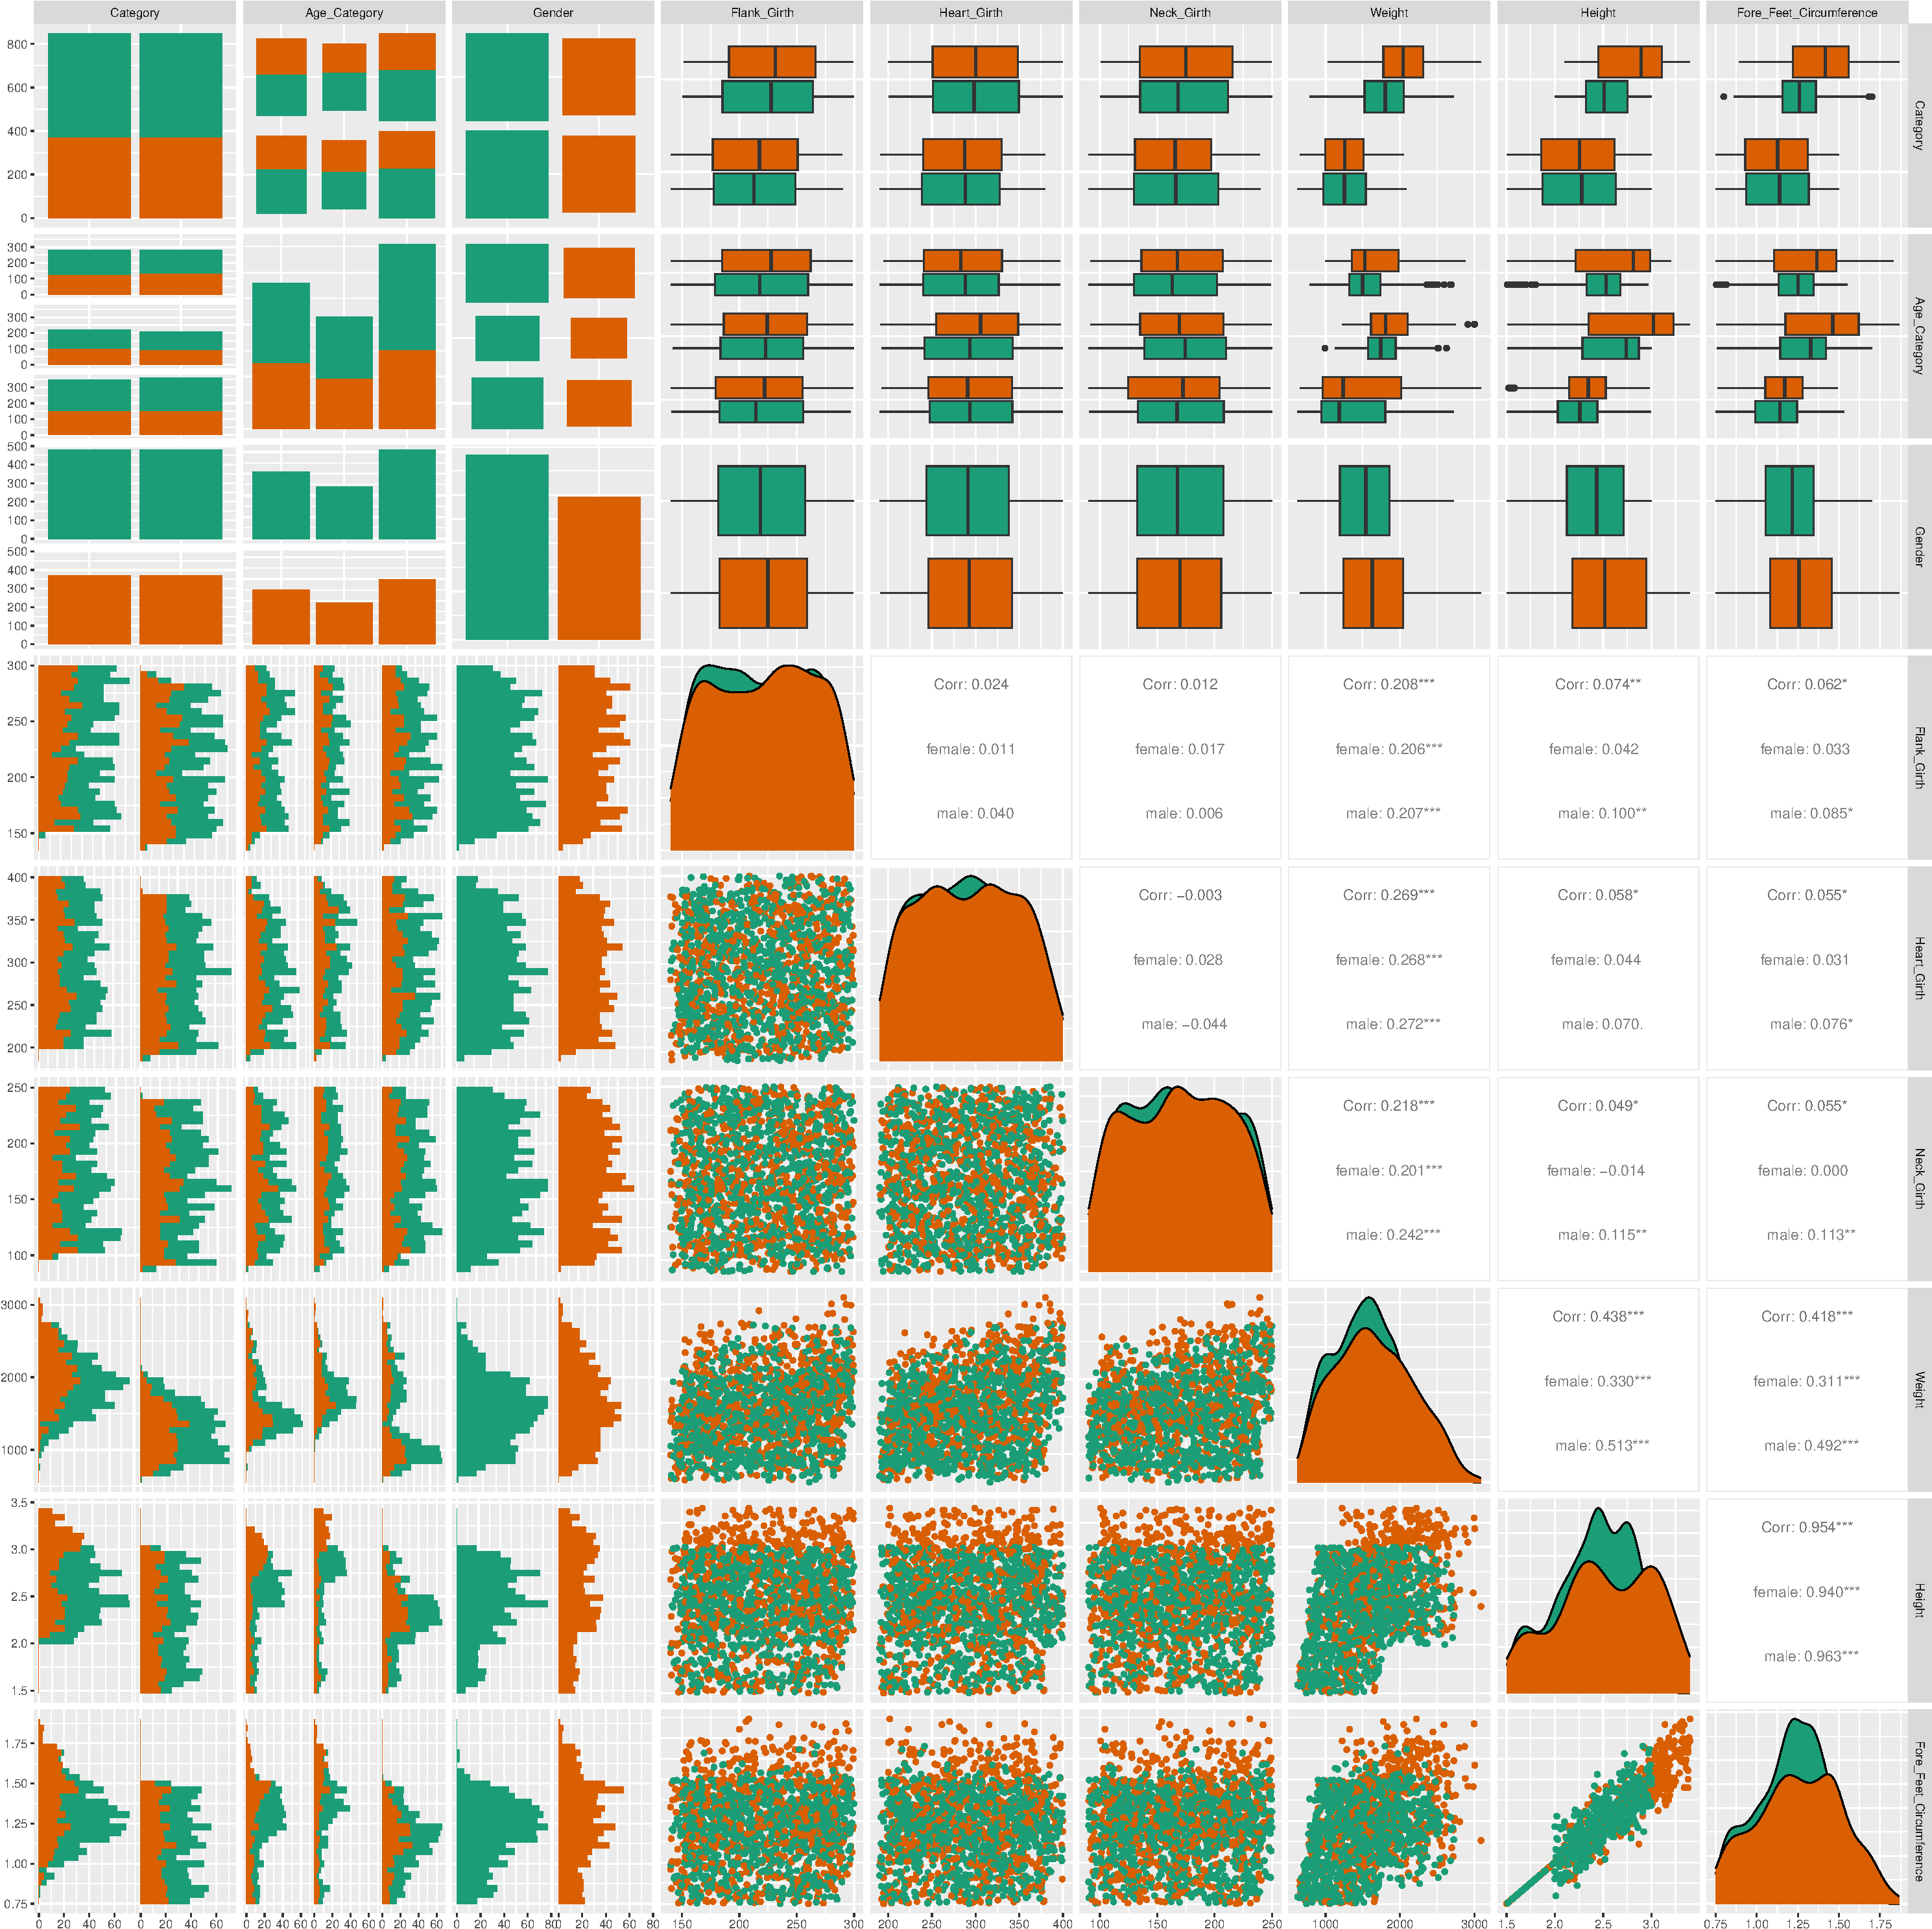
\includegraphics{Data-Visualisation-geom-Encyclopedia_files/figure-latex/unnamed-chunk-9-1.pdf}

\hypertarget{small-cross-sectional-dataset}{%
\section{Small cross sectional dataset}\label{small-cross-sectional-dataset}}

\begin{Shaded}
\begin{Highlighting}[]
\FunctionTok{set.seed}\NormalTok{(}\DecValTok{2023}\NormalTok{)}
\NormalTok{elephants.subset}\FloatTok{.100} \OtherTok{\textless{}{-}}\NormalTok{ elephants }\SpecialCharTok{|}\ErrorTok{\textgreater{}} \FunctionTok{sample\_n}\NormalTok{(}\DecValTok{100}\NormalTok{)}
\end{Highlighting}
\end{Shaded}

\hypertarget{glimpse-of-the-small-cross-sectional-dataset}{%
\subsection{Glimpse of the small cross sectional dataset}\label{glimpse-of-the-small-cross-sectional-dataset}}

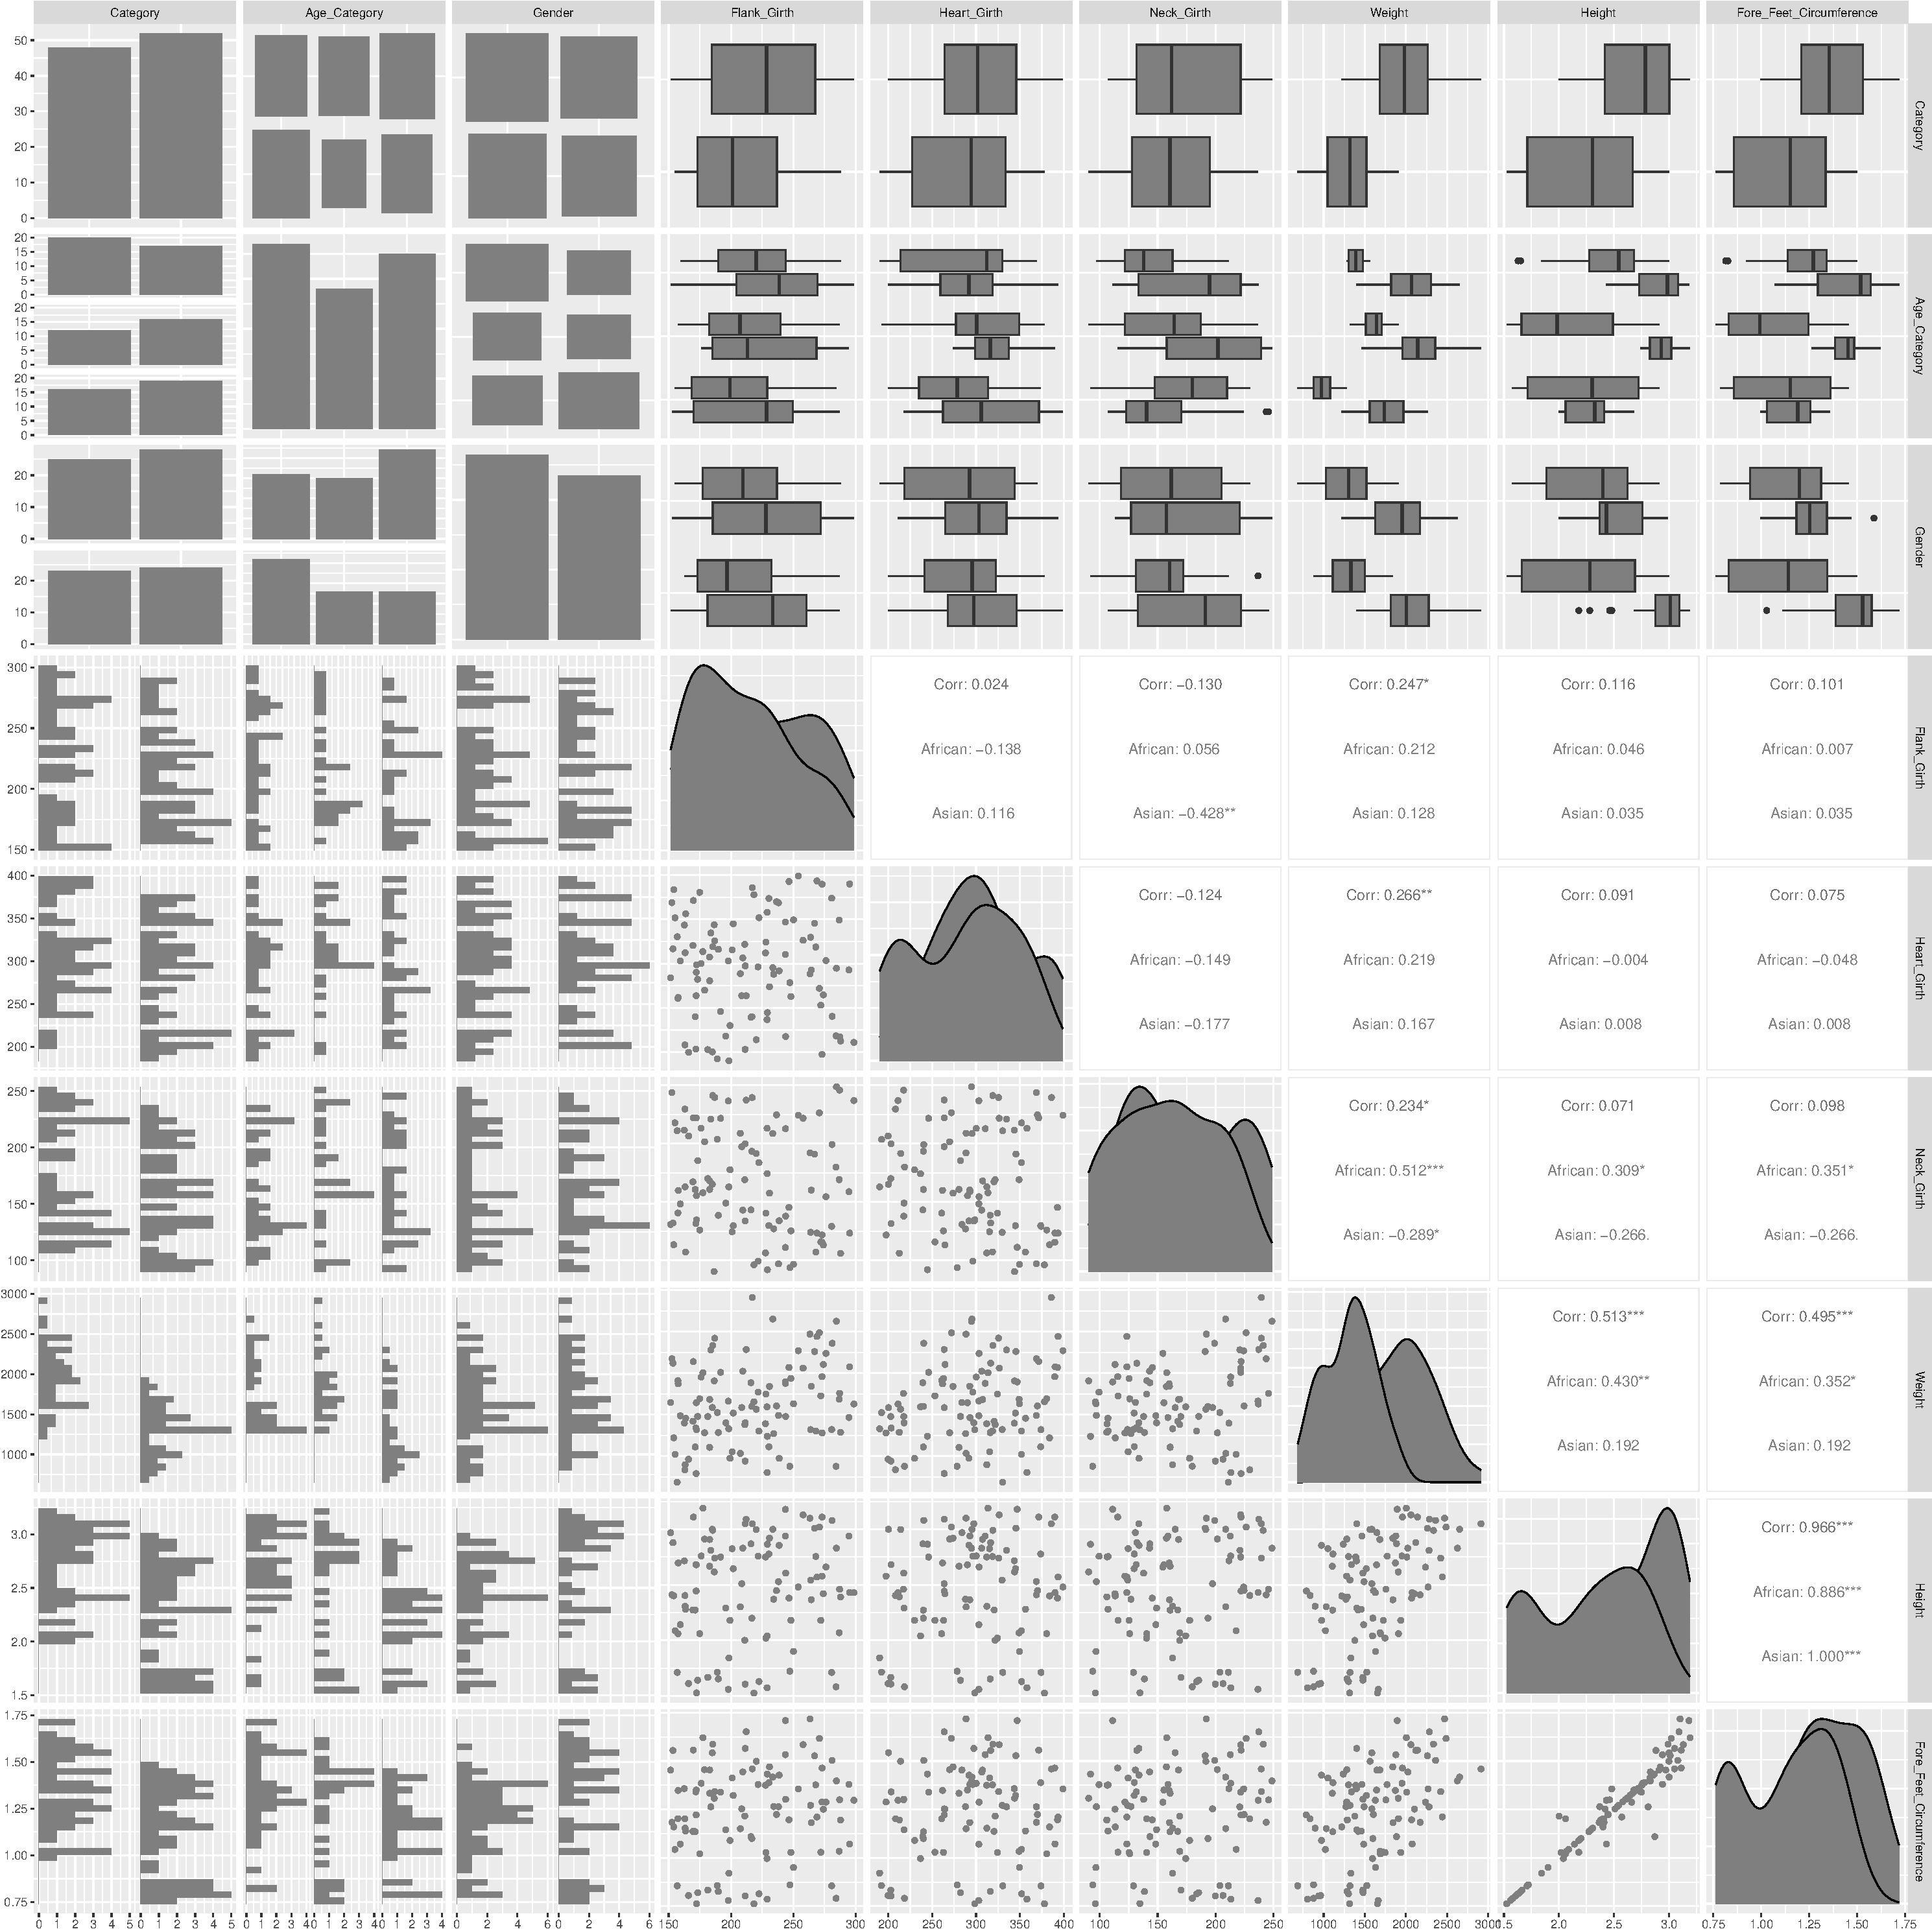
\includegraphics{Data-Visualisation-geom-Encyclopedia_files/figure-latex/unnamed-chunk-11-1.pdf}

\hypertarget{time-series-dataset}{%
\section{Time series dataset}\label{time-series-dataset}}

\begin{Shaded}
\begin{Highlighting}[]
\FunctionTok{library}\NormalTok{(denguedatahub)}
\NormalTok{srilanka\_weekly\_data}
\end{Highlighting}
\end{Shaded}

\begin{verbatim}
## # A tibble: 21,934 x 6
##     year  week start.date end.date   district    cases
##  * <dbl> <dbl> <date>     <date>     <chr>       <dbl>
##  1  2006    52 2006-12-23 2006-12-29 Colombo        71
##  2  2006    52 2006-12-23 2006-12-29 Gampaha        12
##  3  2006    52 2006-12-23 2006-12-29 Kalutara       12
##  4  2006    52 2006-12-23 2006-12-29 Kandy          20
##  5  2006    52 2006-12-23 2006-12-29 Matale          4
##  6  2006    52 2006-12-23 2006-12-29 NuwaraEliya     1
##  7  2006    52 2006-12-23 2006-12-29 Galle           1
##  8  2006    52 2006-12-23 2006-12-29 Hambanthota     1
##  9  2006    52 2006-12-23 2006-12-29 Matara         11
## 10  2006    52 2006-12-23 2006-12-29 Jaffna          0
## # i 21,924 more rows
\end{verbatim}

\hypertarget{packages-related-to-geom}{%
\section{Packages related to geom}\label{packages-related-to-geom}}

\begin{Shaded}
\begin{Highlighting}[]
\FunctionTok{library}\NormalTok{(ggplot2)}
\CommentTok{\#devtools::install\_github("EvaMaeRey/ggxmean")}
\CommentTok{\#library(gxmean)}
\CommentTok{\#devtools::install\_github("davidsjoberg/ggsankey")}
\FunctionTok{library}\NormalTok{(ggxmean)}
\end{Highlighting}
\end{Shaded}

\hypertarget{geom-extensions}{%
\section{geom Extensions}\label{geom-extensions}}

\begin{Shaded}
\begin{Highlighting}[]
\FunctionTok{library}\NormalTok{(GGally) }\CommentTok{\# Matrix plots}
\end{Highlighting}
\end{Shaded}

\hypertarget{all-available-geom_-in-the-ggplot2-package}{%
\section{All available geom\_\ldots{} in the ggplot2 package}\label{all-available-geom_-in-the-ggplot2-package}}

\begin{tabular}{l}
\hline
x\\
\hline
geom\_abline\\
\hline
geom\_area\\
\hline
geom\_bar\\
\hline
geom\_bin\_2d\\
\hline
geom\_bin2d\\
\hline
geom\_blank\\
\hline
geom\_boxplot\\
\hline
geom\_col\\
\hline
geom\_contour\\
\hline
geom\_contour\_filled\\
\hline
geom\_count\\
\hline
geom\_crossbar\\
\hline
geom\_curve\\
\hline
geom\_density\\
\hline
geom\_density\_2d\\
\hline
geom\_density\_2d\_filled\\
\hline
geom\_density2d\\
\hline
geom\_density2d\_filled\\
\hline
geom\_dotplot\\
\hline
geom\_errorbar\\
\hline
geom\_errorbarh\\
\hline
geom\_freqpoly\\
\hline
geom\_function\\
\hline
geom\_hex\\
\hline
geom\_histogram\\
\hline
geom\_hline\\
\hline
geom\_jitter\\
\hline
geom\_label\\
\hline
geom\_line\\
\hline
geom\_linerange\\
\hline
geom\_map\\
\hline
geom\_path\\
\hline
geom\_point\\
\hline
geom\_pointrange\\
\hline
geom\_polygon\\
\hline
geom\_qq\\
\hline
geom\_qq\_line\\
\hline
geom\_quantile\\
\hline
geom\_raster\\
\hline
geom\_rect\\
\hline
geom\_ribbon\\
\hline
geom\_rug\\
\hline
geom\_segment\\
\hline
geom\_sf\\
\hline
geom\_sf\_label\\
\hline
geom\_sf\_text\\
\hline
geom\_smooth\\
\hline
geom\_spoke\\
\hline
geom\_step\\
\hline
geom\_text\\
\hline
geom\_tile\\
\hline
geom\_violin\\
\hline
geom\_vline\\
\hline
\end{tabular}

\hypertarget{a-geom_a}{%
\chapter{A: geom\_a\ldots{}}\label{a-geom_a}}

\hypertarget{abline}{%
\section{geom\_abline}\label{abline}}

\textbf{Package: } ggplot2 \autocite{R-ggplot2}

\textbf{Book: }

\textbf{Description: } Draw a straight line (\(Y=mX+c\)) for a given slope (\(m\)) and intercept (\(c\)).

\textbf{See also: } \protect\hyperlink{point}{geom\_point}, \protect\hyperlink{vline}{geom\_vline}, \protect\hyperlink{hline}{geom\_hline}

\textbf{Example:}

\begin{Shaded}
\begin{Highlighting}[]
\NormalTok{abline }\OtherTok{\textless{}{-}} \FunctionTok{ggplot}\NormalTok{(elephants.subset}\FloatTok{.100}\NormalTok{, }\FunctionTok{aes}\NormalTok{(}\AttributeTok{y =}\NormalTok{ Height, }\AttributeTok{x=}\NormalTok{Fore\_Feet\_Circumference)) }\SpecialCharTok{+} \FunctionTok{geom\_abline}\NormalTok{(}\AttributeTok{intercept =} \FloatTok{0.15}\NormalTok{, }\AttributeTok{slope =} \FloatTok{1.9}\NormalTok{) }\SpecialCharTok{+} 
  \FunctionTok{labs}\NormalTok{(}\AttributeTok{title=}\StringTok{"A: \textasciigrave{}geom\_abline\textasciigrave{} only"}\NormalTok{) }\SpecialCharTok{+}
  \FunctionTok{theme}\NormalTok{(}\AttributeTok{aspect.ratio =} \DecValTok{1}\NormalTok{)}

\NormalTok{pointabline }\OtherTok{\textless{}{-}} \FunctionTok{ggplot}\NormalTok{(elephants.subset}\FloatTok{.100}\NormalTok{, }\FunctionTok{aes}\NormalTok{(}\AttributeTok{y =}\NormalTok{ Height, }\AttributeTok{x=}\NormalTok{Fore\_Feet\_Circumference)) }\SpecialCharTok{+} 
  \FunctionTok{geom\_point}\NormalTok{() }\SpecialCharTok{+} 
  \FunctionTok{geom\_abline}\NormalTok{(}\AttributeTok{intercept =} \FloatTok{0.15}\NormalTok{, }\AttributeTok{slope =} \FloatTok{1.9}\NormalTok{) }\SpecialCharTok{+} 
  \FunctionTok{labs}\NormalTok{(}\AttributeTok{title=}\StringTok{"B: \textasciigrave{}geom\_point + geom\_abline\textasciigrave{} both"}\NormalTok{) }\SpecialCharTok{+}
  \FunctionTok{theme}\NormalTok{(}\AttributeTok{aspect.ratio =} \DecValTok{1}\NormalTok{)}

\FunctionTok{library}\NormalTok{(patchwork)}
\NormalTok{abline }\SpecialCharTok{|}\NormalTok{ pointabline}
\end{Highlighting}
\end{Shaded}

\begin{figure}
\centering
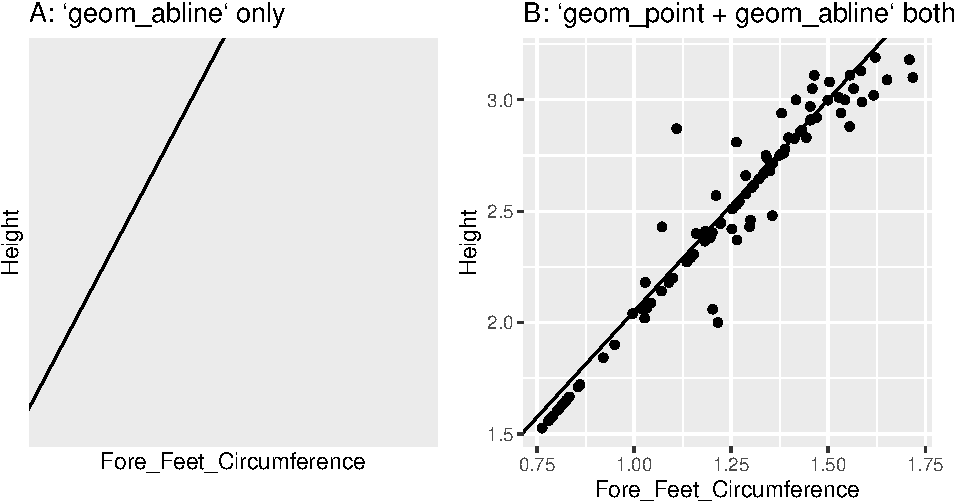
\includegraphics{Data-Visualisation-geom-Encyclopedia_files/figure-latex/unnamed-chunk-16-1.pdf}
\caption{\label{fig:unnamed-chunk-16}Illustration of (A) geom\_abline and (B) use of geom\_point and geom\_abline both}
\end{figure}

\hypertarget{area}{%
\section{geom\_area}\label{area}}

\textbf{Package: } ggplot2 \autocite{R-ggplot2}

\textbf{Description: }Create an area plot. This cover the space between x-axis and line that connects the data points.

\textbf{See also: } \protect\hyperlink{line}{geom\_line}

\begin{Shaded}
\begin{Highlighting}[]
\NormalTok{colombo }\OtherTok{\textless{}{-}}\NormalTok{ srilanka\_weekly\_data }\SpecialCharTok{|}\ErrorTok{\textgreater{}}
  \FunctionTok{filter}\NormalTok{(district }\SpecialCharTok{==} \StringTok{"Colombo"}\NormalTok{)}
\FunctionTok{ggplot}\NormalTok{(}\AttributeTok{data=}\NormalTok{colombo, }\FunctionTok{aes}\NormalTok{(}\AttributeTok{x=}\NormalTok{start.date, }\AttributeTok{y=}\NormalTok{cases)) }\SpecialCharTok{+} 
  \FunctionTok{geom\_area}\NormalTok{()}
\end{Highlighting}
\end{Shaded}

\begin{figure}
\centering
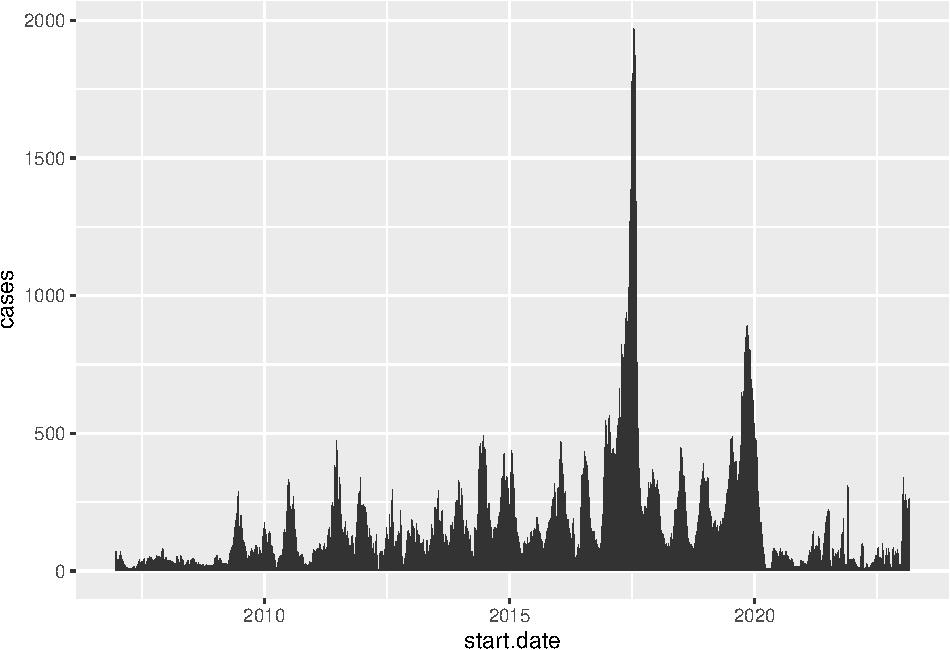
\includegraphics{Data-Visualisation-geom-Encyclopedia_files/figure-latex/unnamed-chunk-17-1.pdf}
\caption{\label{fig:unnamed-chunk-17}Illustration of geom\_area}
\end{figure}

\hypertarget{b-geom_b}{%
\chapter{B: geom\_b\ldots{}}\label{b-geom_b}}

\hypertarget{geom_bar}{%
\section{geom\_bar}\label{geom_bar}}

\textbf{Package: } ggplot2 \autocite{R-ggplot2}

\textbf{Description: } Draw a bar proportional to the specified number. For example, number of cases or user defined number.

\textbf{Statistics layer(s): }

\texttt{stat\_count} - This the default statistics layer. It counts number of cases in each group.

\texttt{stat\_identify} - It plots the data as it is.

\textbf{See also: } \protect\hyperlink{col}{geom\_col}

\hypertarget{with-count}{%
\subsection{With count}\label{with-count}}

\begin{Shaded}
\begin{Highlighting}[]
\FunctionTok{ggplot}\NormalTok{(elephants, }\FunctionTok{aes}\NormalTok{(}\AttributeTok{y =}\NormalTok{ Age\_Category)) }\SpecialCharTok{+} 
  \FunctionTok{geom\_bar}\NormalTok{()}
\end{Highlighting}
\end{Shaded}

\begin{figure}
\centering
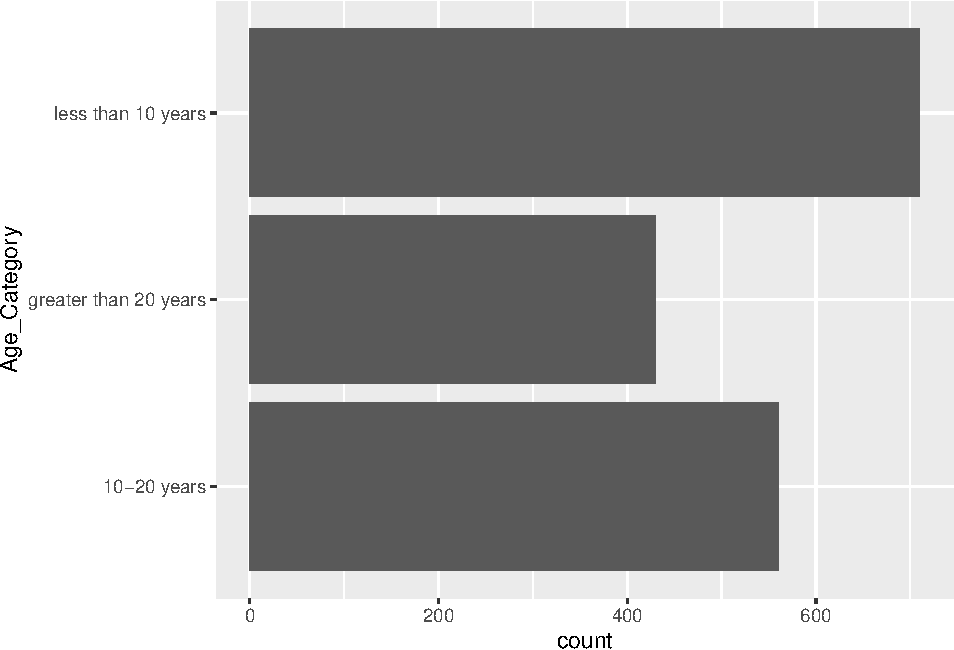
\includegraphics{Data-Visualisation-geom-Encyclopedia_files/figure-latex/unnamed-chunk-18-1.pdf}
\caption{\label{fig:unnamed-chunk-18}Illustration of geom\_bar to create a bar chart}
\end{figure}

\begin{Shaded}
\begin{Highlighting}[]
\FunctionTok{ggplot}\NormalTok{(elephants, }\FunctionTok{aes}\NormalTok{(}\AttributeTok{y =}\NormalTok{ Age\_Category, }\AttributeTok{fill=}\NormalTok{Category)) }\SpecialCharTok{+} 
  \FunctionTok{geom\_bar}\NormalTok{()}
\end{Highlighting}
\end{Shaded}

\begin{figure}
\centering
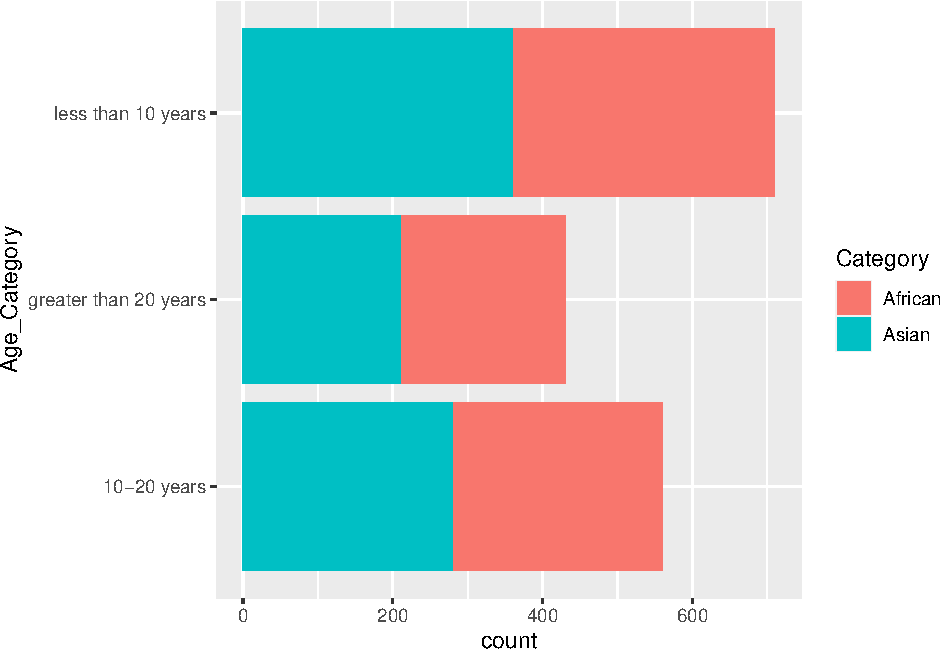
\includegraphics{Data-Visualisation-geom-Encyclopedia_files/figure-latex/unnamed-chunk-19-1.pdf}
\caption{\label{fig:unnamed-chunk-19}Illustration of geom\_bar to create a stacked bar chart}
\end{figure}

\begin{Shaded}
\begin{Highlighting}[]
\FunctionTok{ggplot}\NormalTok{(elephants, }\FunctionTok{aes}\NormalTok{(}\AttributeTok{y=}\NormalTok{Age\_Category, }\AttributeTok{fill =}\NormalTok{ Category)) }\SpecialCharTok{+}
  \FunctionTok{geom\_bar}\NormalTok{(}\AttributeTok{position =} \StringTok{"dodge"}\NormalTok{)}
\end{Highlighting}
\end{Shaded}

\begin{figure}
\centering
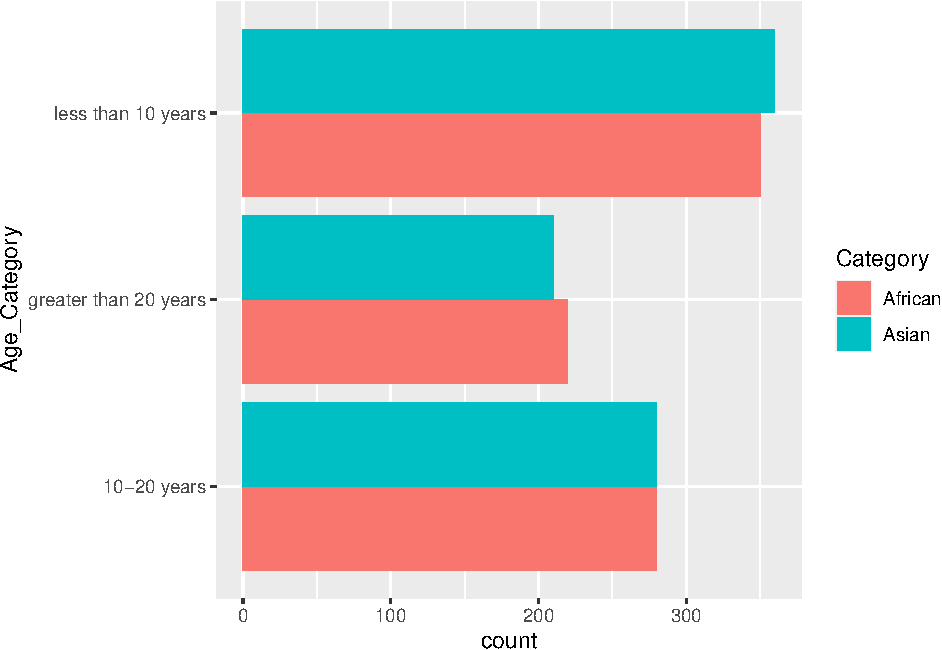
\includegraphics{Data-Visualisation-geom-Encyclopedia_files/figure-latex/unnamed-chunk-20-1.pdf}
\caption{\label{fig:unnamed-chunk-20}Illustration of geom\_bar to create a cluster bar chart}
\end{figure}

\begin{Shaded}
\begin{Highlighting}[]
\FunctionTok{ggplot}\NormalTok{(elephants, }\FunctionTok{aes}\NormalTok{(}\AttributeTok{y=}\NormalTok{Age\_Category, }\AttributeTok{fill =}\NormalTok{ Category)) }\SpecialCharTok{+}
  \FunctionTok{geom\_bar}\NormalTok{(}\AttributeTok{position =} \StringTok{"dodge"}\NormalTok{)}
\end{Highlighting}
\end{Shaded}

\begin{figure}
\centering
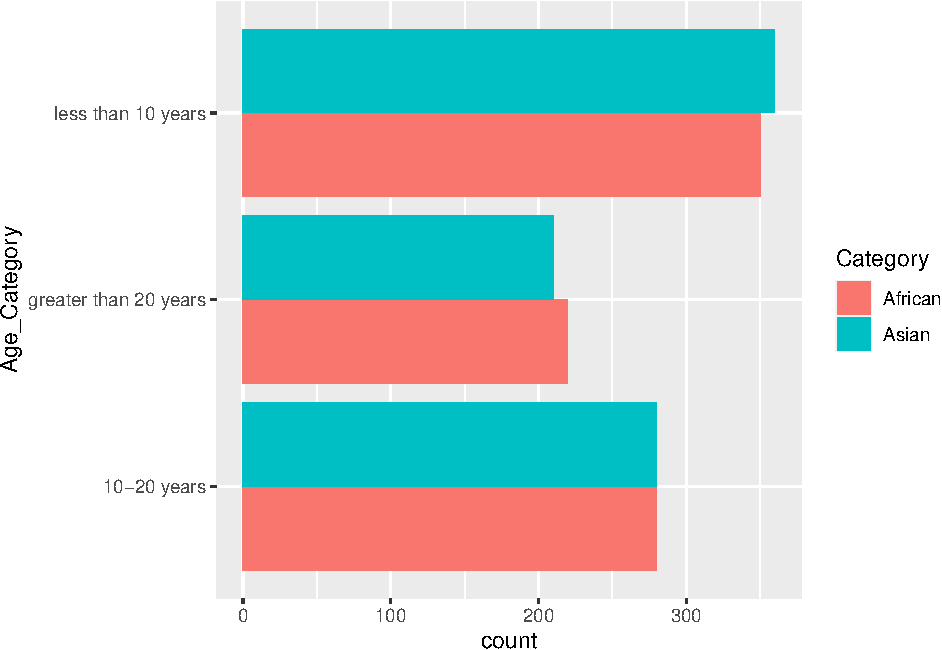
\includegraphics{Data-Visualisation-geom-Encyclopedia_files/figure-latex/unnamed-chunk-21-1.pdf}
\caption{\label{fig:unnamed-chunk-21}Illustration of geom\_bar to create a cluster bar chart}
\end{figure}

\hypertarget{with-identity}{%
\subsection{With identity}\label{with-identity}}

\begin{Shaded}
\begin{Highlighting}[]
\NormalTok{dfbar }\OtherTok{\textless{}{-}} \FunctionTok{data.frame}\NormalTok{(}\AttributeTok{class=}\FunctionTok{c}\NormalTok{(}\StringTok{"A"}\NormalTok{, }\StringTok{"B"}\NormalTok{),  }\AttributeTok{income =} \FunctionTok{c}\NormalTok{(}\DecValTok{100}\NormalTok{, }\DecValTok{200}\NormalTok{))}
\FunctionTok{ggplot}\NormalTok{(dfbar, }\FunctionTok{aes}\NormalTok{(class, income)) }\SpecialCharTok{+}
  \FunctionTok{geom\_bar}\NormalTok{(}\AttributeTok{stat=}\StringTok{"identity"}\NormalTok{)}
\end{Highlighting}
\end{Shaded}

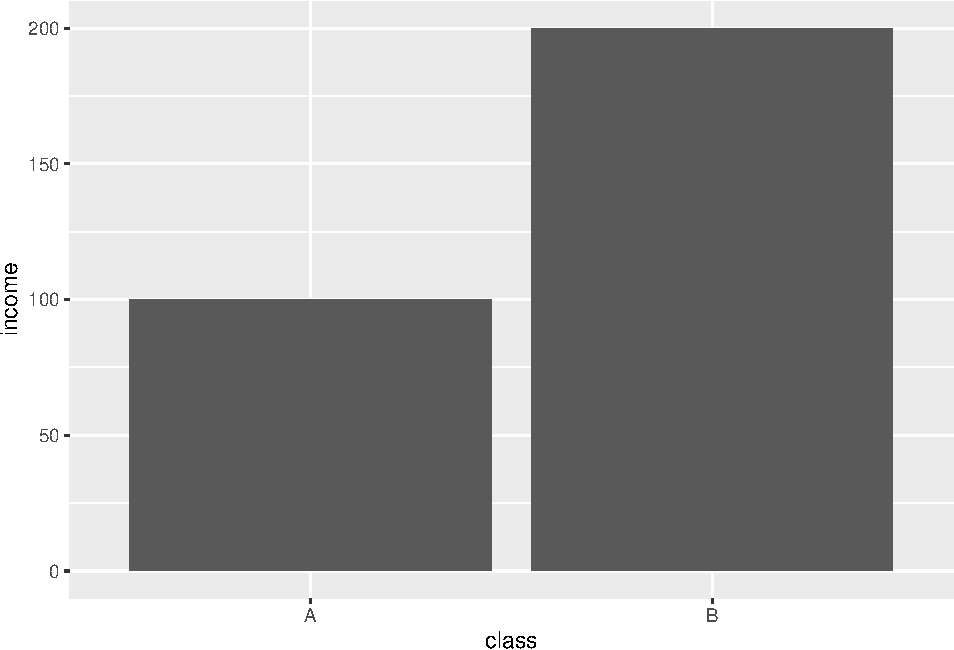
\includegraphics{Data-Visualisation-geom-Encyclopedia_files/figure-latex/unnamed-chunk-22-1.pdf}

\hypertarget{geom_bin_2d}{%
\section{geom\_bin\_2d}\label{geom_bin_2d}}

\textbf{Package: } ggplot2 \autocite{R-ggplot2}

\textbf{Description: } Divides the Cartesian plane created by x-variable and y-variable into rectangles, counts the number of observations in each rectangle. Only the observations with rectangles are filled according to the number ofobservations.

\textbf{Understandable aesthetics: } x, y, fill, group

\textbf{Statistics layer(s): }

\textbf{See also: } \protect\hyperlink{bin2d}{geom\_bin2d}, \protect\hyperlink{point}{geom\_point}

\begin{Shaded}
\begin{Highlighting}[]
\FunctionTok{ggplot}\NormalTok{(elephants.subset}\FloatTok{.100}\NormalTok{, }\FunctionTok{aes}\NormalTok{(}\AttributeTok{y =}\NormalTok{ Height, }\AttributeTok{x=}\NormalTok{Fore\_Feet\_Circumference)) }\SpecialCharTok{+}
  \FunctionTok{geom\_bin\_2d}\NormalTok{() }\SpecialCharTok{+} 
  \FunctionTok{theme}\NormalTok{(}\AttributeTok{aspect.ratio =} \DecValTok{1}\NormalTok{)}
\end{Highlighting}
\end{Shaded}

\begin{figure}
\centering
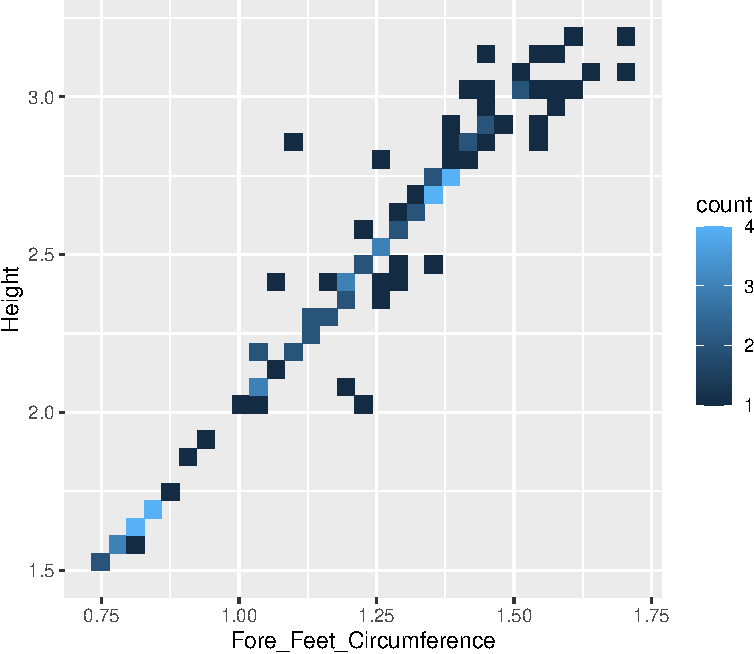
\includegraphics{Data-Visualisation-geom-Encyclopedia_files/figure-latex/unnamed-chunk-23-1.pdf}
\caption{\label{fig:unnamed-chunk-23}Illustration of using geom\_bin\_2d}
\end{figure}

\begin{Shaded}
\begin{Highlighting}[]
\FunctionTok{ggplot}\NormalTok{(elephants.subset}\FloatTok{.100}\NormalTok{, }\FunctionTok{aes}\NormalTok{(}\AttributeTok{y =}\NormalTok{ Height, }\AttributeTok{x=}\NormalTok{Fore\_Feet\_Circumference)) }\SpecialCharTok{+}
  \FunctionTok{geom\_bin\_2d}\NormalTok{(}\AttributeTok{bins=}\DecValTok{20}\NormalTok{) }\SpecialCharTok{+} 
  \FunctionTok{theme}\NormalTok{(}\AttributeTok{aspect.ratio =} \DecValTok{1}\NormalTok{)}
\end{Highlighting}
\end{Shaded}

\begin{figure}
\centering
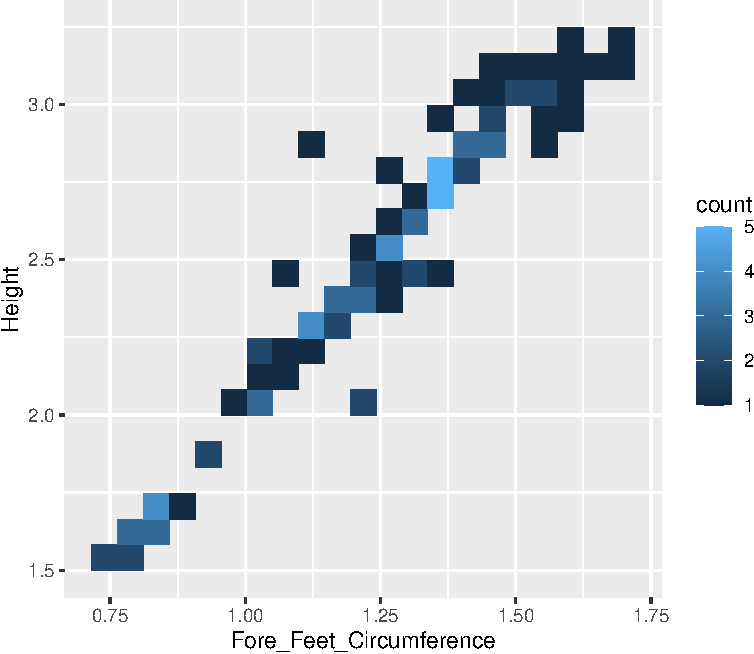
\includegraphics{Data-Visualisation-geom-Encyclopedia_files/figure-latex/unnamed-chunk-24-1.pdf}
\caption{\label{fig:unnamed-chunk-24}Illustration of changing bins in geom\_bin\_2d}
\end{figure}

\hypertarget{geom_bin2d}{%
\section{geom\_bin2d}\label{geom_bin2d}}

\textbf{Package: } ggplot2 \autocite{R-ggplot2}

\textbf{Description: } Divides the Cartesian plane created by x-variable and y-variable into rectangles, counts the number of observations in each rectangle. Only the observations with rectangles are filled according to the number ofobservations.

\textbf{Understandable aesthetics: } x, y, fill, group

\textbf{Statistics layer(s): }

\textbf{See also: } \protect\hyperlink{bin_2d}{geom\_bin\_2d}, \protect\hyperlink{point}{geom\_point}

\textbf{Example:}

\begin{Shaded}
\begin{Highlighting}[]
\FunctionTok{ggplot}\NormalTok{(elephants.subset}\FloatTok{.100}\NormalTok{, }\FunctionTok{aes}\NormalTok{(}\AttributeTok{y =}\NormalTok{ Height, }\AttributeTok{x=}\NormalTok{Fore\_Feet\_Circumference)) }\SpecialCharTok{+}
  \FunctionTok{geom\_bin2d}\NormalTok{() }\SpecialCharTok{+} 
  \FunctionTok{theme}\NormalTok{(}\AttributeTok{aspect.ratio =} \DecValTok{1}\NormalTok{)}
\end{Highlighting}
\end{Shaded}

\begin{figure}
\centering
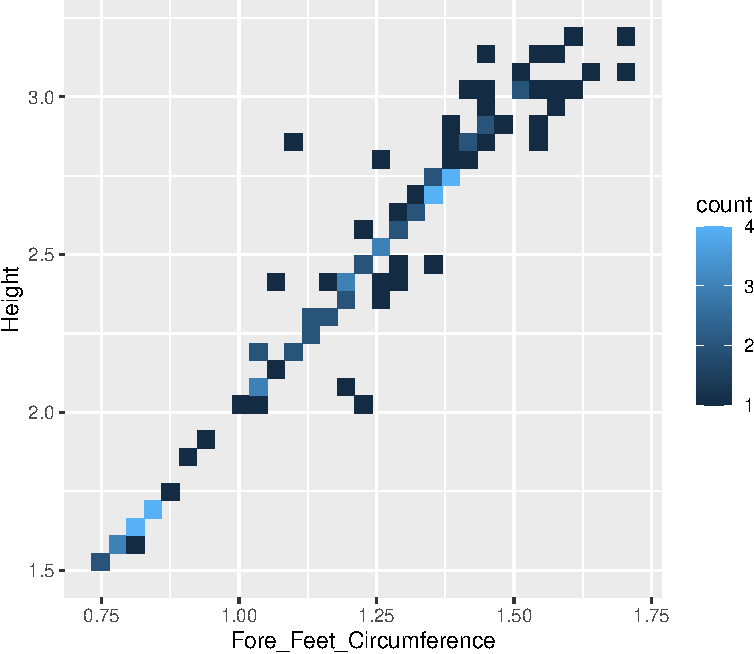
\includegraphics{Data-Visualisation-geom-Encyclopedia_files/figure-latex/unnamed-chunk-25-1.pdf}
\caption{\label{fig:unnamed-chunk-25}Illustration of using geom\_bin\_2d}
\end{figure}

\hypertarget{geom_blank}{%
\section{geom\_blank}\label{geom_blank}}

\textbf{Package: } ggplot2 \autocite{R-ggplot2}

\textbf{Description: } Draws nothing.

\hypertarget{geom_boxplot}{%
\section{geom\_boxplot}\label{geom_boxplot}}

\textbf{Package: } ggplot2 \autocite{R-ggplot2}

\textbf{Description: } Draw a bar proportional to the specified number. For example, number of cases or user defined number.

\textbf{Statistics layer(s): }

\texttt{stat\_boxplot} - This the default statistics layer. This computes minimum, maximum, median, first quartile (\(Q1\)), third quartile (\(Q3\)), upper whisker extends up to \(Q3 + 1.5 \times IQR\) and lower whisker extends up to \(Q1 - 1.5 \times IQR\), where \(IQR = Q3 - Q1\). In a notched box plot, it creates 95\% confidence interval for mean.

\textbf{See also: } \protect\hyperlink{col}{geom\_col}

\begin{Shaded}
\begin{Highlighting}[]
\FunctionTok{ggplot}\NormalTok{(elephants, }\FunctionTok{aes}\NormalTok{(}\AttributeTok{y =}\NormalTok{ Weight)) }\SpecialCharTok{+} 
  \FunctionTok{geom\_boxplot}\NormalTok{()}
\end{Highlighting}
\end{Shaded}

\begin{figure}
\centering
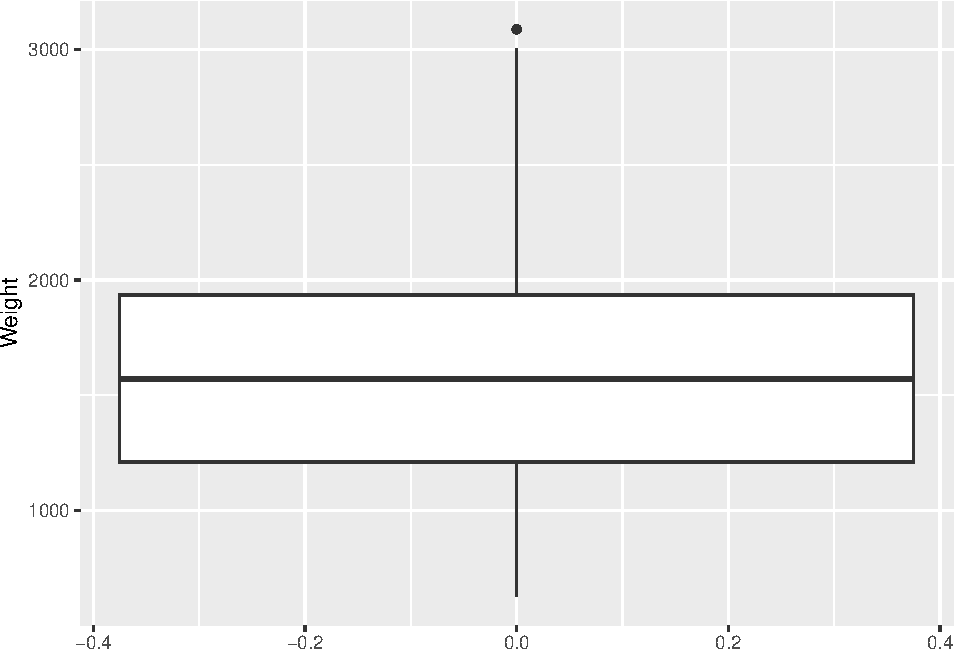
\includegraphics{Data-Visualisation-geom-Encyclopedia_files/figure-latex/unnamed-chunk-26-1.pdf}
\caption{\label{fig:unnamed-chunk-26}Illustration of using geom\_boxplot}
\end{figure}

\begin{Shaded}
\begin{Highlighting}[]
\FunctionTok{ggplot}\NormalTok{(elephants, }\FunctionTok{aes}\NormalTok{(}\AttributeTok{y =}\NormalTok{ Weight)) }\SpecialCharTok{+} 
\FunctionTok{geom\_boxplot}\NormalTok{(}\AttributeTok{outlier.colour=}\StringTok{"black"}\NormalTok{, }\AttributeTok{outlier.shape=}\DecValTok{16}\NormalTok{,}
             \AttributeTok{outlier.size=}\DecValTok{2}\NormalTok{, }\AttributeTok{notch=}\ConstantTok{TRUE}\NormalTok{)}
\end{Highlighting}
\end{Shaded}

\begin{figure}
\centering
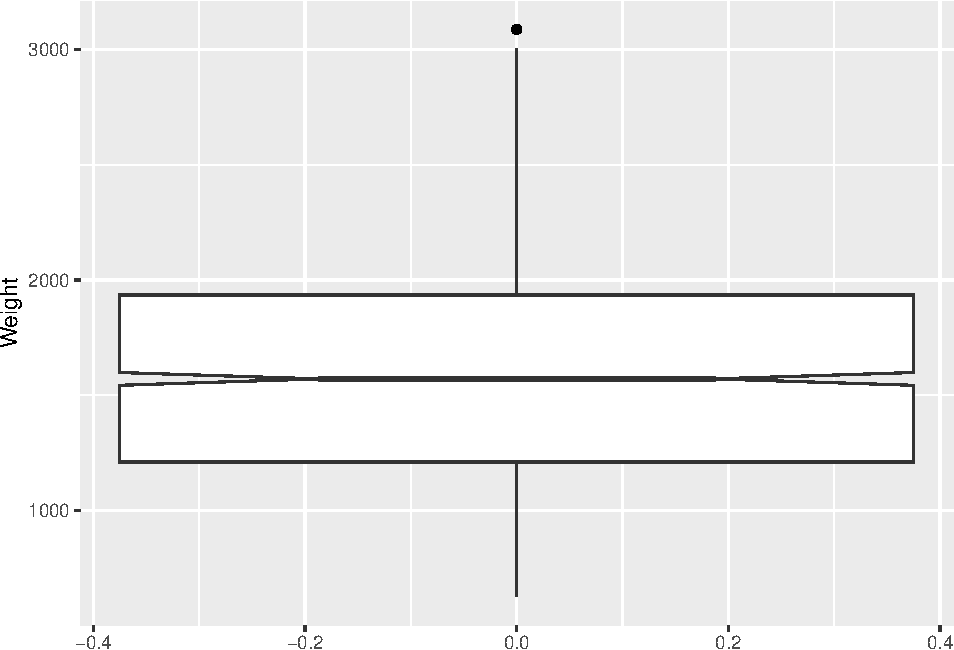
\includegraphics{Data-Visualisation-geom-Encyclopedia_files/figure-latex/unnamed-chunk-27-1.pdf}
\caption{\label{fig:unnamed-chunk-27}Illustration of using geom\_boxplot with changing outliers and adding a notch to create notched box plot.}
\end{figure}

\hypertarget{c-geom_c}{%
\chapter{C: geom\_c\ldots{}}\label{c-geom_c}}

\hypertarget{geom_col}{%
\section{geom\_col}\label{geom_col}}

Before using \texttt{geom\_col}, you need to create a summary table of counts or you can apply \texttt{geom\_col} for a summary table already given.

\begin{verbatim}
## # A tibble: 3 x 2
##   Age_Category              n
##   <chr>                 <int>
## 1 10-20 years             560
## 2 greater than 20 years   430
## 3 less than 10 years      710
\end{verbatim}

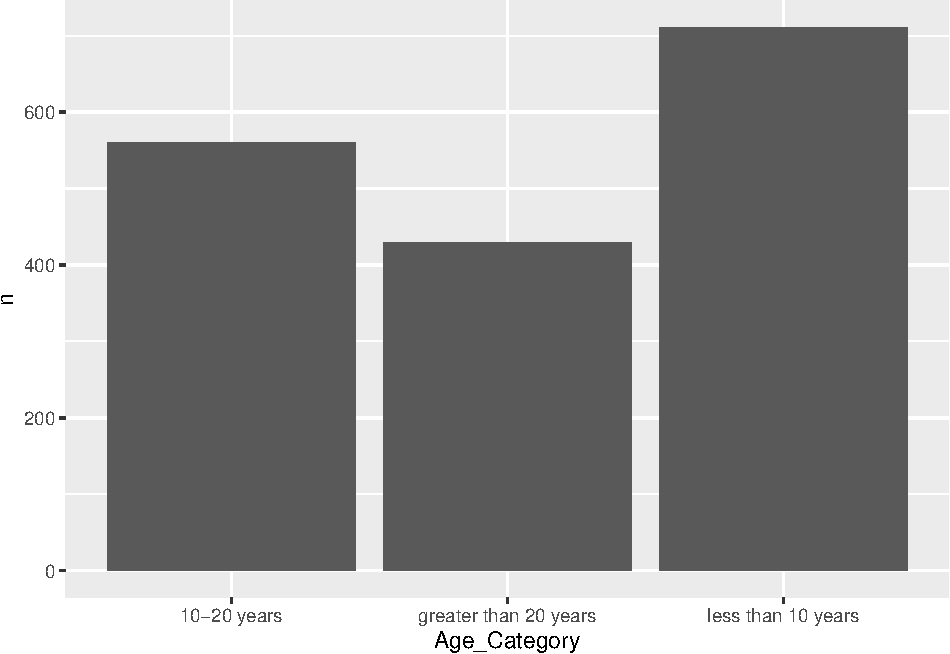
\includegraphics{Data-Visualisation-geom-Encyclopedia_files/figure-latex/unnamed-chunk-29-1.pdf}

\hypertarget{d-geom_d}{%
\chapter{D: geom\_d\ldots{}}\label{d-geom_d}}

\hypertarget{geom_delaunay_tile}{%
\section{geom\_delaunay\_tile}\label{geom_delaunay_tile}}

\textbf{Description:} The Delaunay triangulation is used to create a planar graph.

\begin{Shaded}
\begin{Highlighting}[]
\NormalTok{delaunay }\OtherTok{\textless{}{-}} \FunctionTok{ggplot}\NormalTok{(elephants.subset}\FloatTok{.100}\NormalTok{, }\FunctionTok{aes}\NormalTok{(}\AttributeTok{y =}\NormalTok{ Height, }\AttributeTok{x=}\NormalTok{Fore\_Feet\_Circumference)) }\SpecialCharTok{+}
\NormalTok{  ggforce}\SpecialCharTok{::}\FunctionTok{geom\_delaunay\_tile}\NormalTok{(}\AttributeTok{alpha =} \FloatTok{0.5}\NormalTok{, }\AttributeTok{colour =} \StringTok{\textquotesingle{}black\textquotesingle{}}\NormalTok{) }\SpecialCharTok{+} \FunctionTok{labs}\NormalTok{(}\AttributeTok{title=}\StringTok{"geom\_delaunay\_tile"}\NormalTok{) }\SpecialCharTok{+} \FunctionTok{theme}\NormalTok{(}\AttributeTok{aspect.ratio =} \DecValTok{1}\NormalTok{)}

\CommentTok{\# to compare with geom\_point}
\NormalTok{point }\OtherTok{\textless{}{-}} \FunctionTok{ggplot}\NormalTok{(elephants.subset}\FloatTok{.100}\NormalTok{, }\FunctionTok{aes}\NormalTok{(}\AttributeTok{y =}\NormalTok{ Height, }\AttributeTok{x=}\NormalTok{Fore\_Feet\_Circumference)) }\SpecialCharTok{+}
  \FunctionTok{geom\_point}\NormalTok{(}\AttributeTok{alpha =} \FloatTok{0.5}\NormalTok{, }\AttributeTok{colour =} \StringTok{\textquotesingle{}black\textquotesingle{}}\NormalTok{) }\SpecialCharTok{+} \FunctionTok{labs}\NormalTok{(}\AttributeTok{title=}\StringTok{"geom\_point"}\NormalTok{) }\SpecialCharTok{+} \FunctionTok{theme}\NormalTok{(}\AttributeTok{aspect.ratio =} \DecValTok{1}\NormalTok{)}

\FunctionTok{library}\NormalTok{(patchwork)}
\NormalTok{delaunay}\SpecialCharTok{|}\NormalTok{point}
\end{Highlighting}
\end{Shaded}

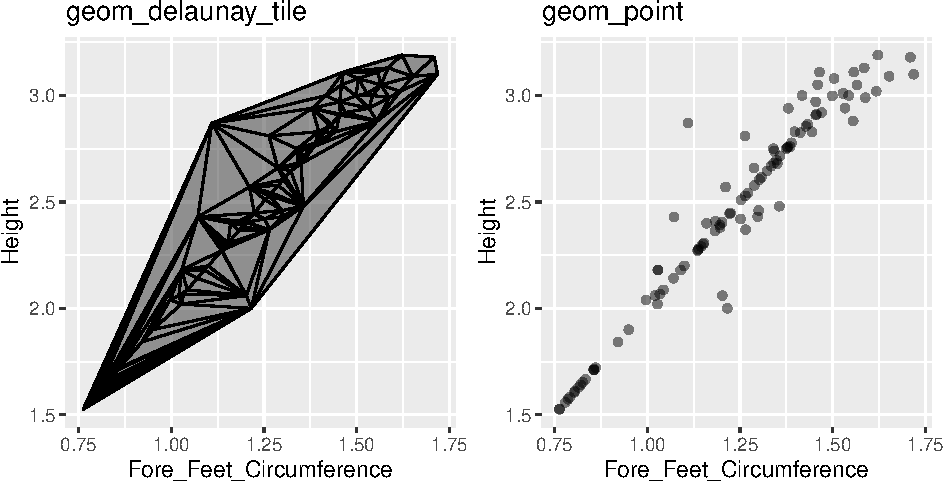
\includegraphics{Data-Visualisation-geom-Encyclopedia_files/figure-latex/unnamed-chunk-30-1.pdf}

\hypertarget{geom_density}{%
\section{geom\_density}\label{geom_density}}

\begin{Shaded}
\begin{Highlighting}[]
\FunctionTok{ggplot}\NormalTok{(elephants, }\FunctionTok{aes}\NormalTok{(}\AttributeTok{x =}\NormalTok{ Weight)) }\SpecialCharTok{+} 
  \FunctionTok{geom\_density}\NormalTok{()}
\end{Highlighting}
\end{Shaded}

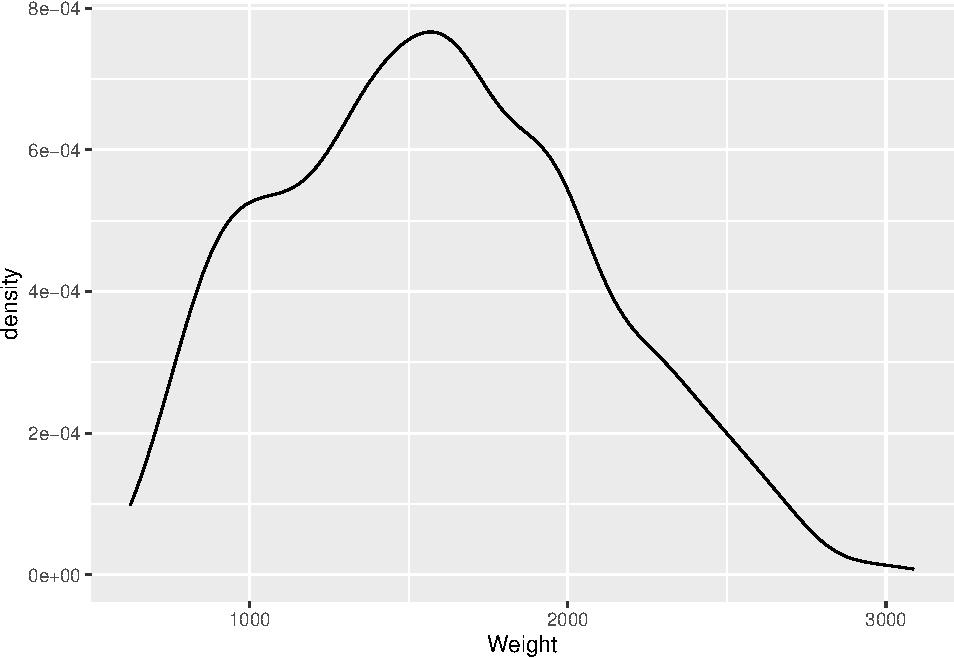
\includegraphics{Data-Visualisation-geom-Encyclopedia_files/figure-latex/unnamed-chunk-31-1.pdf}

\hypertarget{geom_density_2d}{%
\section{geom\_density\_2d}\label{geom_density_2d}}

\begin{Shaded}
\begin{Highlighting}[]
\FunctionTok{ggplot}\NormalTok{(elephants, }\FunctionTok{aes}\NormalTok{(}\AttributeTok{y =}\NormalTok{ Height, }\AttributeTok{x=}\NormalTok{Weight)) }\SpecialCharTok{+} 
  \FunctionTok{geom\_density\_2d}\NormalTok{()}
\end{Highlighting}
\end{Shaded}

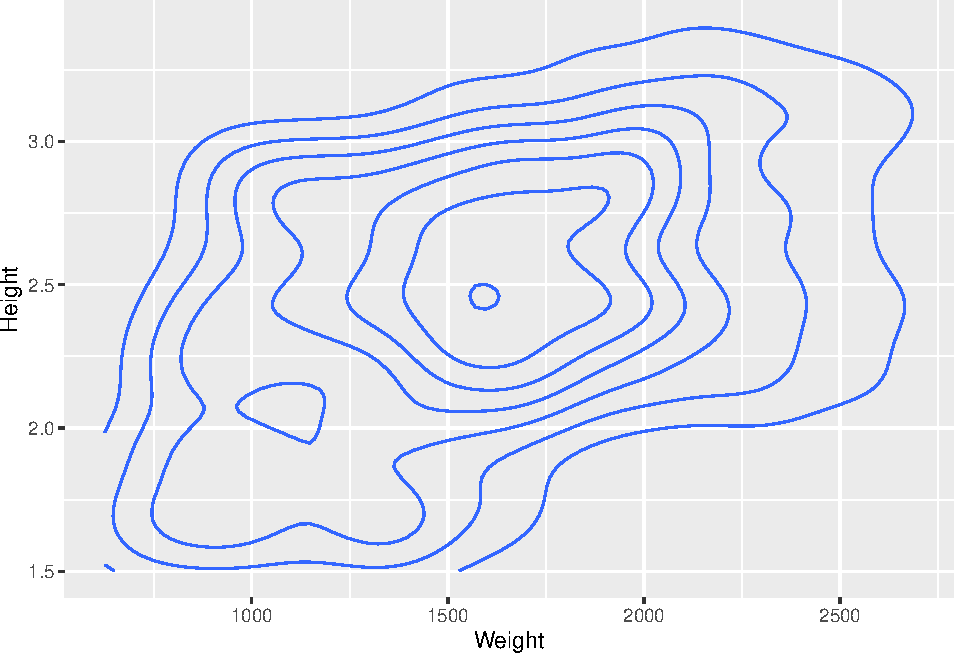
\includegraphics{Data-Visualisation-geom-Encyclopedia_files/figure-latex/unnamed-chunk-32-1.pdf}

\hypertarget{geom_density_2d_filled}{%
\section{geom\_density\_2d\_filled}\label{geom_density_2d_filled}}

\begin{Shaded}
\begin{Highlighting}[]
\FunctionTok{ggplot}\NormalTok{(elephants, }\FunctionTok{aes}\NormalTok{(}\AttributeTok{y =}\NormalTok{ Height, }\AttributeTok{x=}\NormalTok{Weight)) }\SpecialCharTok{+} 
  \FunctionTok{geom\_density\_2d\_filled}\NormalTok{()}
\end{Highlighting}
\end{Shaded}

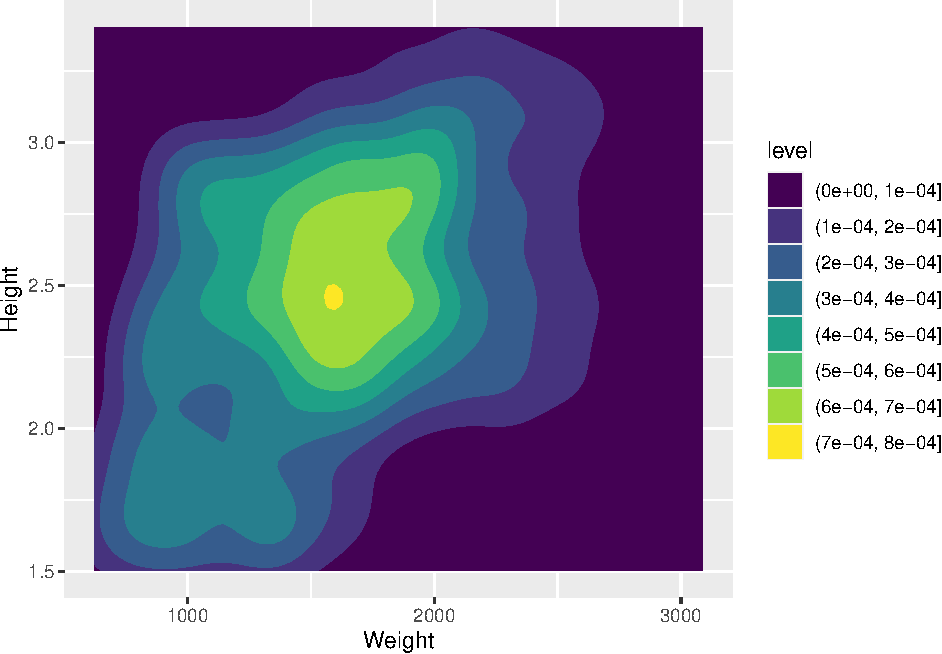
\includegraphics{Data-Visualisation-geom-Encyclopedia_files/figure-latex/unnamed-chunk-33-1.pdf}

\hypertarget{geom_density_ridges}{%
\section{geom\_density\_ridges}\label{geom_density_ridges}}

Here the \texttt{y} variable should be qualitative and the \texttt{x} variable should be quantitative.

\begin{Shaded}
\begin{Highlighting}[]
\FunctionTok{library}\NormalTok{(ggridges)}
\FunctionTok{ggplot}\NormalTok{(elephants, }\FunctionTok{aes}\NormalTok{(}\AttributeTok{y=}\NormalTok{Category, }\AttributeTok{x =}\NormalTok{ Height)) }\SpecialCharTok{+} 
    \FunctionTok{geom\_density\_ridges}\NormalTok{()}
\end{Highlighting}
\end{Shaded}

\begin{verbatim}
## Picking joint bandwidth of 0.092
\end{verbatim}

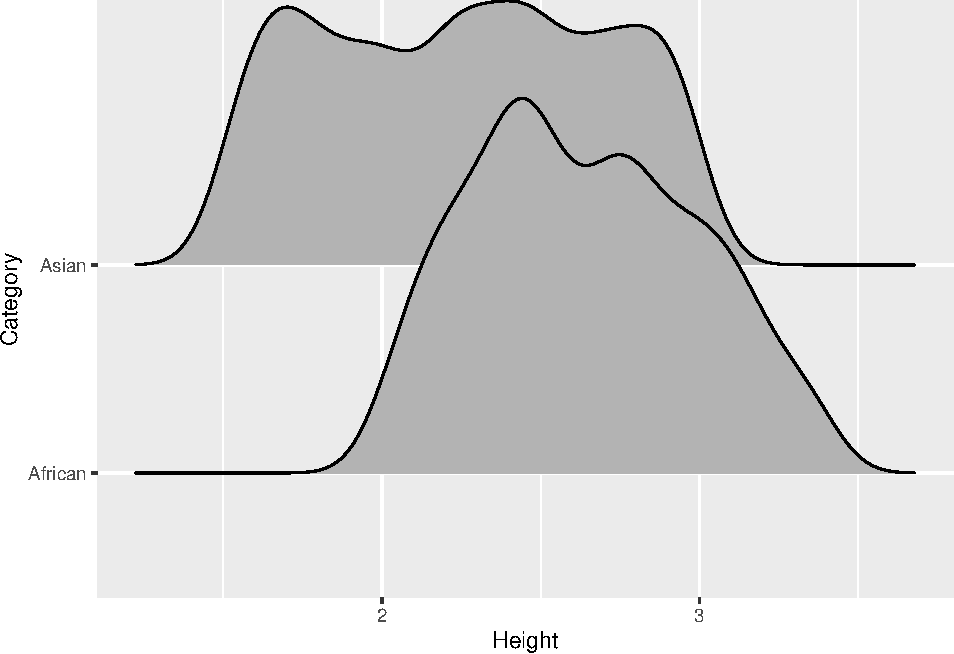
\includegraphics{Data-Visualisation-geom-Encyclopedia_files/figure-latex/unnamed-chunk-34-1.pdf}

\hypertarget{geom_dl}{%
\section{geom\_dl}\label{geom_dl}}

\begin{Shaded}
\begin{Highlighting}[]
\FunctionTok{library}\NormalTok{(directlabels)}
\FunctionTok{ggplot}\NormalTok{(elephants, }\FunctionTok{aes}\NormalTok{(}\AttributeTok{y =}\NormalTok{ Height, }\AttributeTok{x=}\NormalTok{Weight, }\AttributeTok{col=}\NormalTok{Category)) }\SpecialCharTok{+} 
  \FunctionTok{geom\_point}\NormalTok{() }\SpecialCharTok{+}
  \FunctionTok{geom\_dl}\NormalTok{(}\FunctionTok{aes}\NormalTok{(}\AttributeTok{label=}\NormalTok{Category),}\AttributeTok{method=}\StringTok{"smart.grid"}\NormalTok{)}
\end{Highlighting}
\end{Shaded}

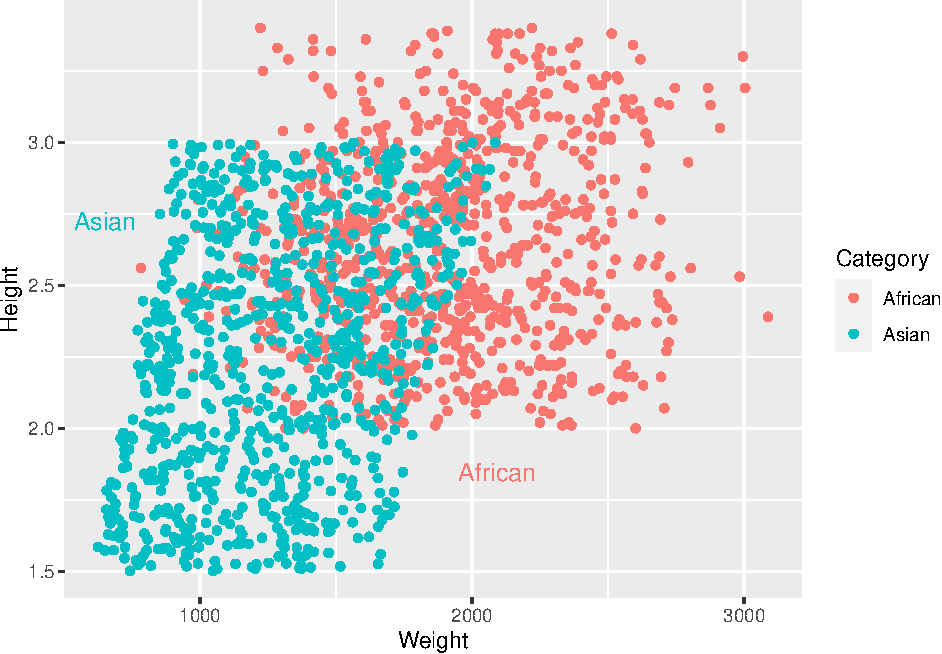
\includegraphics{Data-Visualisation-geom-Encyclopedia_files/figure-latex/unnamed-chunk-35-1.pdf}

\hypertarget{e-geom_e}{%
\chapter{E: geom\_e\ldots{}}\label{e-geom_e}}

\hypertarget{geom_encircle}{%
\section{geom\_encircle}\label{geom_encircle}}

Other related geoms: geom\_mark\_circle

\begin{verbatim}
## Registered S3 methods overwritten by 'ggalt':
##   method                  from   
##   grid.draw.absoluteGrob  ggplot2
##   grobHeight.absoluteGrob ggplot2
##   grobWidth.absoluteGrob  ggplot2
##   grobX.absoluteGrob      ggplot2
##   grobY.absoluteGrob      ggplot2
\end{verbatim}

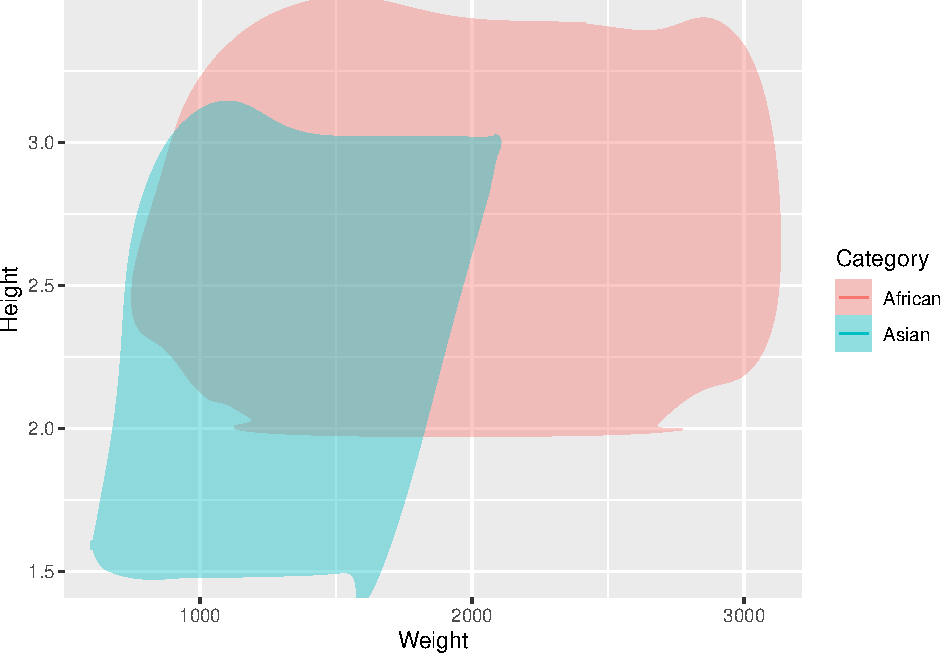
\includegraphics{Data-Visualisation-geom-Encyclopedia_files/figure-latex/unnamed-chunk-36-1.pdf}

\texttt{geom\_encircle} with \texttt{geom\_point}

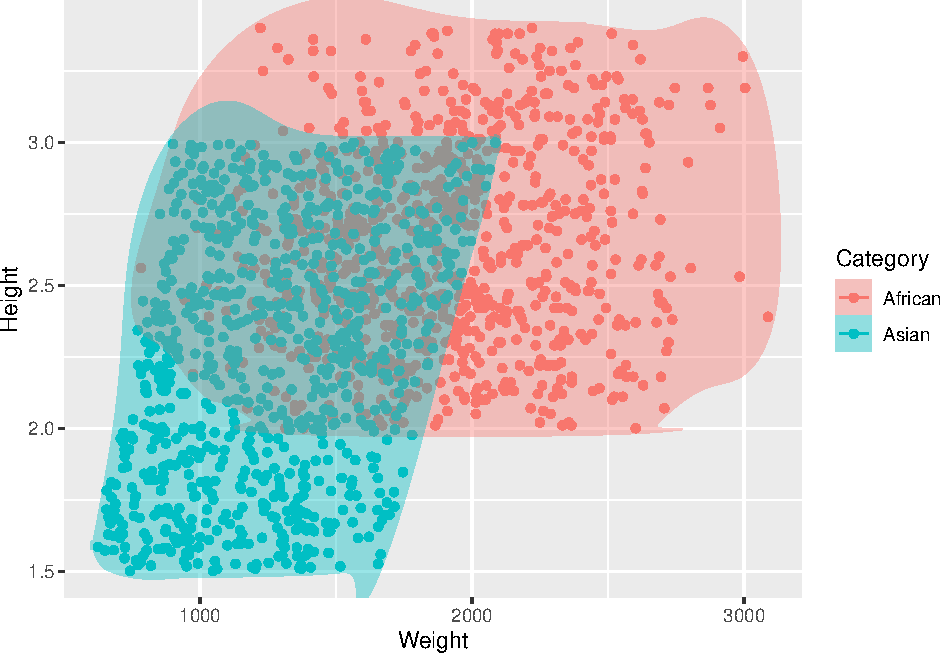
\includegraphics{Data-Visualisation-geom-Encyclopedia_files/figure-latex/unnamed-chunk-37-1.pdf}

\hypertarget{f-geom_f}{%
\chapter{F: geom\_f\ldots{}}\label{f-geom_f}}

\hypertarget{geom_function}{%
\section{geom\_function}\label{geom_function}}

\begin{Shaded}
\begin{Highlighting}[]
\FunctionTok{ggplot}\NormalTok{() }\SpecialCharTok{+} \FunctionTok{xlim}\NormalTok{(}\FunctionTok{c}\NormalTok{(}\SpecialCharTok{{-}}\DecValTok{1}\NormalTok{,}\DecValTok{1}\NormalTok{)) }\SpecialCharTok{+} \FunctionTok{geom\_function}\NormalTok{(}\AttributeTok{fun=}\NormalTok{cos, }\AttributeTok{colour=}\StringTok{"red"}\NormalTok{,}\AttributeTok{lwd=}\DecValTok{1}\NormalTok{, }\AttributeTok{linetype=}\DecValTok{1}\NormalTok{)}
\end{Highlighting}
\end{Shaded}

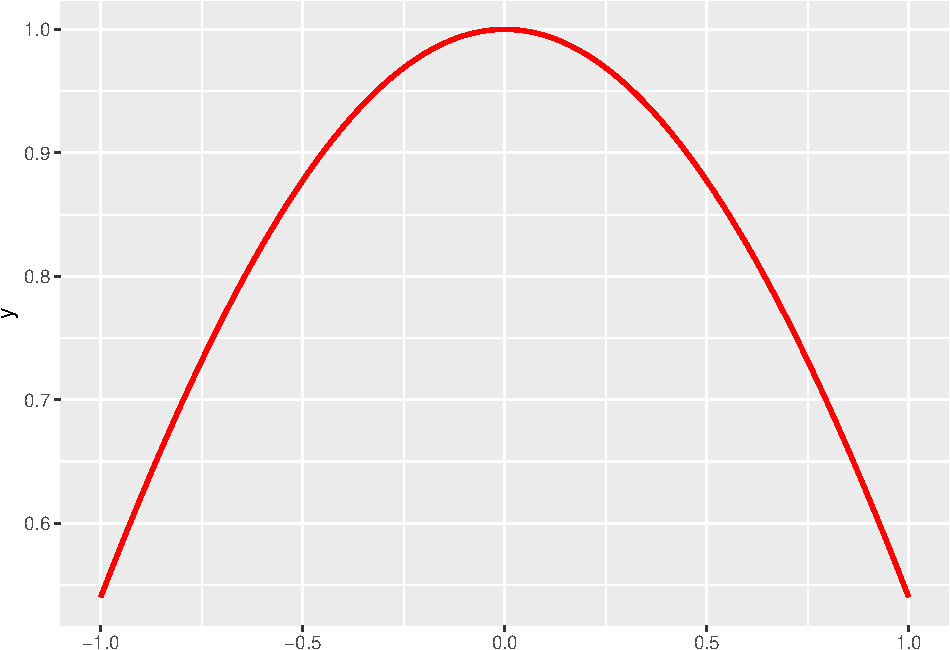
\includegraphics{Data-Visualisation-geom-Encyclopedia_files/figure-latex/unnamed-chunk-38-1.pdf}

\hypertarget{a-geom_axxxxx}{%
\chapter{A: geom\_axxxxx}\label{a-geom_axxxxx}}

\hypertarget{h-geom_h}{%
\chapter{H: geom\_h\ldots{}}\label{h-geom_h}}

\hypertarget{histogram}{%
\section{geom\_histogram}\label{histogram}}

\begin{verbatim}
## `stat_bin()` using `bins = 30`. Pick better value with `binwidth`.
\end{verbatim}

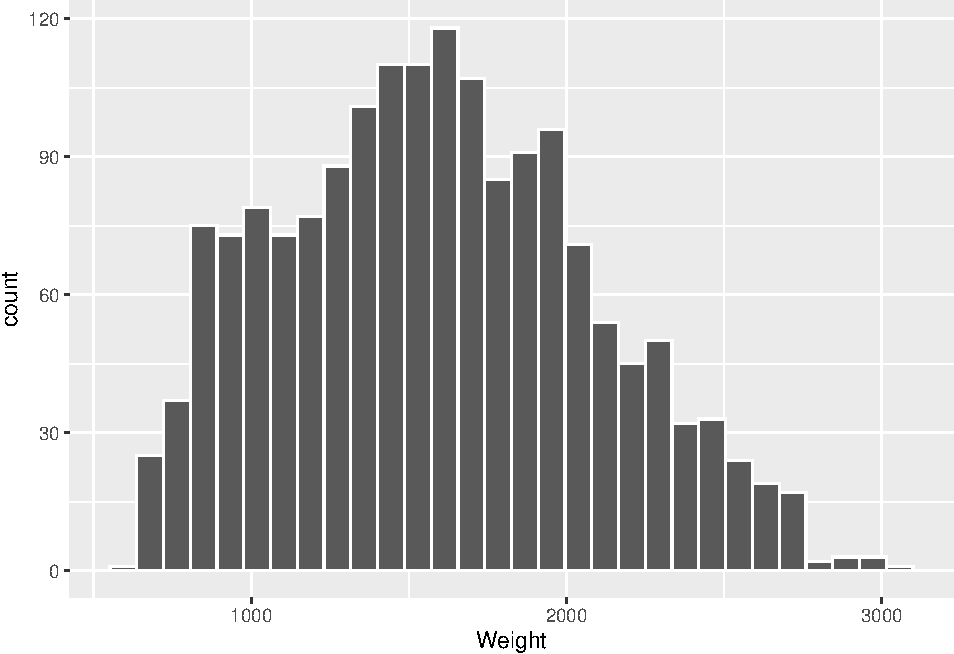
\includegraphics{Data-Visualisation-geom-Encyclopedia_files/figure-latex/unnamed-chunk-39-1.pdf}

\hypertarget{hline}{%
\section{geom\_hline}\label{hline}}

\textbf{Package: } ggplot2 \autocite{R-ggplot2}

\textbf{Book: }

\textbf{Description: } Draw a horizontal line (\(Y=c\)) for a given value of \(c\), which is known as \texttt{yintercept}.

\textbf{See also: } \protect\hyperlink{point}{geom\_point}, \protect\hyperlink{vline}{geom\_vline}, \protect\hyperlink{hline}{geom\_hline}

\textbf{Example:}

\begin{Shaded}
\begin{Highlighting}[]
\NormalTok{hline }\OtherTok{\textless{}{-}} \FunctionTok{ggplot}\NormalTok{(elephants.subset}\FloatTok{.100}\NormalTok{, }\FunctionTok{aes}\NormalTok{(}\AttributeTok{y =}\NormalTok{ Height, }\AttributeTok{x=}\NormalTok{Fore\_Feet\_Circumference)) }\SpecialCharTok{+} \FunctionTok{geom\_hline}\NormalTok{(}\AttributeTok{yintercept =} \FloatTok{2.5}\NormalTok{) }\SpecialCharTok{+} 
  \FunctionTok{labs}\NormalTok{(}\AttributeTok{title=}\StringTok{"A: \textasciigrave{}geom\_hline\textasciigrave{} only"}\NormalTok{) }\SpecialCharTok{+}
  \FunctionTok{theme}\NormalTok{(}\AttributeTok{aspect.ratio =} \DecValTok{1}\NormalTok{)}

\NormalTok{pointhline }\OtherTok{\textless{}{-}} \FunctionTok{ggplot}\NormalTok{(elephants.subset}\FloatTok{.100}\NormalTok{, }\FunctionTok{aes}\NormalTok{(}\AttributeTok{y =}\NormalTok{ Height, }\AttributeTok{x=}\NormalTok{Fore\_Feet\_Circumference)) }\SpecialCharTok{+} 
  \FunctionTok{geom\_point}\NormalTok{() }\SpecialCharTok{+} 
  \FunctionTok{geom\_hline}\NormalTok{(}\AttributeTok{yintercept =} \FloatTok{2.5}\NormalTok{) }\SpecialCharTok{+} 
  \FunctionTok{labs}\NormalTok{(}\AttributeTok{title=}\StringTok{"B: \textasciigrave{}geom\_point + geom\_hline\textasciigrave{} both"}\NormalTok{) }\SpecialCharTok{+}
  \FunctionTok{theme}\NormalTok{(}\AttributeTok{aspect.ratio =} \DecValTok{1}\NormalTok{)}


\NormalTok{hline }\SpecialCharTok{|}\NormalTok{ pointhline}
\end{Highlighting}
\end{Shaded}

\begin{figure}
\centering
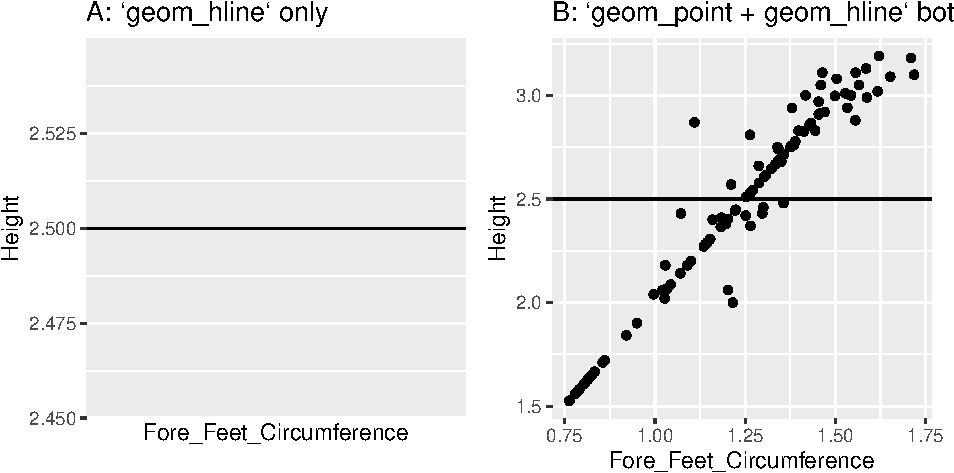
\includegraphics{Data-Visualisation-geom-Encyclopedia_files/figure-latex/unnamed-chunk-40-1.pdf}
\caption{\label{fig:unnamed-chunk-40}Illustration of (A) geom\_hline and (B) use of geom\_point and geom\_hline both}
\end{figure}

\hypertarget{a-geom_axxxxx-1}{%
\chapter{A: geom\_axxxxx}\label{a-geom_axxxxx-1}}

\hypertarget{a-geom_axxxxx-2}{%
\chapter{A: geom\_axxxxx}\label{a-geom_axxxxx-2}}

\hypertarget{a-geom_axxxxx-3}{%
\chapter{A: geom\_axxxxx}\label{a-geom_axxxxx-3}}

\hypertarget{l-geom_l}{%
\chapter{L: geom\_l\ldots{}}\label{l-geom_l}}

\hypertarget{geom_label_repel}{%
\section{geom\_label\_repel}\label{geom_label_repel}}

\begin{Shaded}
\begin{Highlighting}[]
\FunctionTok{ggplot}\NormalTok{(elephants.subset}\FloatTok{.100}\NormalTok{, }\FunctionTok{aes}\NormalTok{(}\AttributeTok{y =}\NormalTok{ Height, }\AttributeTok{x=}\NormalTok{Weight)) }\SpecialCharTok{+}
  \FunctionTok{geom\_point}\NormalTok{() }\SpecialCharTok{+}
\NormalTok{  ggrepel}\SpecialCharTok{::}\FunctionTok{geom\_label\_repel}\NormalTok{(}\FunctionTok{aes}\NormalTok{(}\AttributeTok{y =}\NormalTok{ Height, }\AttributeTok{x=}\NormalTok{Weight, }
                                \AttributeTok{label =} \FunctionTok{rownames}\NormalTok{(elephants.subset}\FloatTok{.100}\NormalTok{)),}
                                \AttributeTok{fontface =} \StringTok{\textquotesingle{}bold\textquotesingle{}}\NormalTok{, }\AttributeTok{color =} \StringTok{\textquotesingle{}red\textquotesingle{}}\NormalTok{,}
                                \AttributeTok{box.padding =} \FunctionTok{unit}\NormalTok{(}\FloatTok{0.40}\NormalTok{, }\StringTok{"lines"}\NormalTok{),}
                                \AttributeTok{point.padding =} \FunctionTok{unit}\NormalTok{(}\FloatTok{0.6}\NormalTok{, }\StringTok{"lines"}\NormalTok{),}
                                \AttributeTok{segment.color =} \StringTok{\textquotesingle{}grey50\textquotesingle{}}
\NormalTok{  )}
\end{Highlighting}
\end{Shaded}

\begin{verbatim}
## Warning: ggrepel: 5 unlabeled data points (too many overlaps). Consider
## increasing max.overlaps
\end{verbatim}

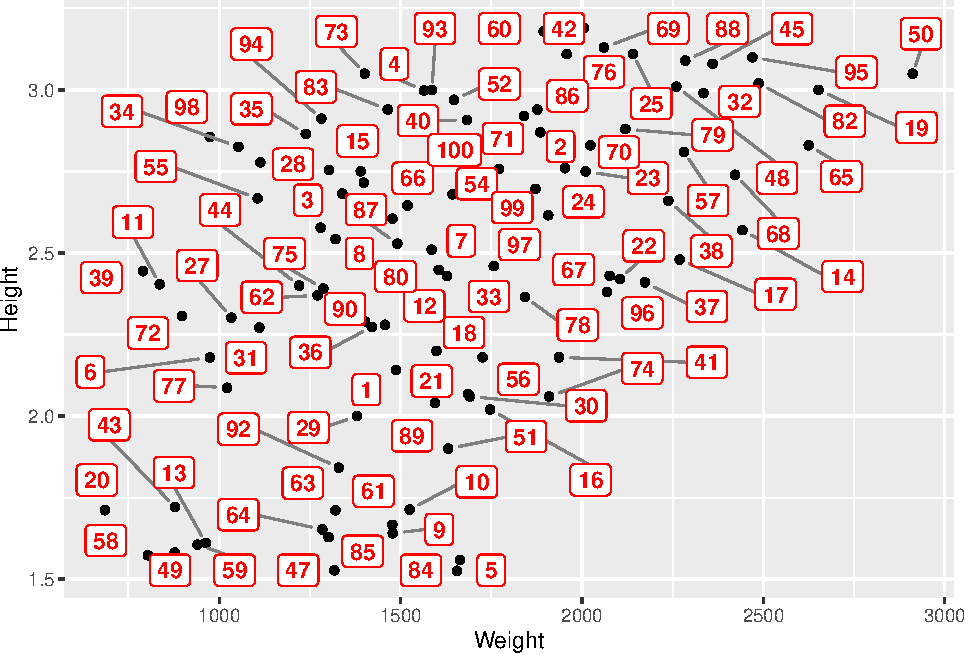
\includegraphics{Data-Visualisation-geom-Encyclopedia_files/figure-latex/unnamed-chunk-41-1.pdf}

\hypertarget{geom_lm}{%
\section{geom\_lm}\label{geom_lm}}

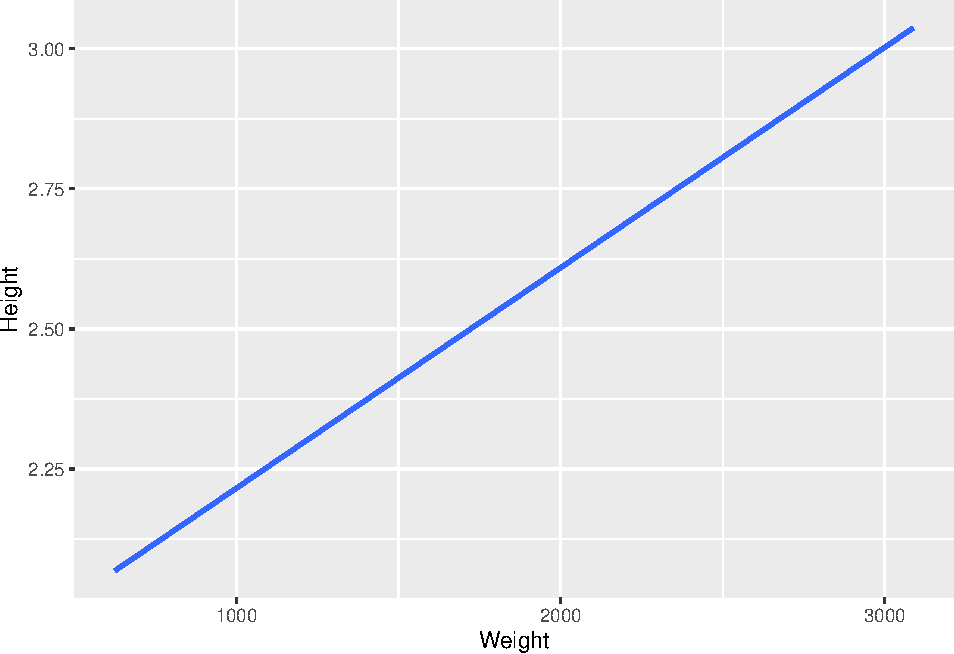
\includegraphics{Data-Visualisation-geom-Encyclopedia_files/figure-latex/unnamed-chunk-42-1.pdf}

\hypertarget{m-geom_m}{%
\chapter{M: geom\_m\ldots{}}\label{m-geom_m}}

\hypertarget{geom_mark_circle}{%
\section{geom\_mark\_circle}\label{geom_mark_circle}}

\begin{verbatim}
## Warning: Using the `size` aesthetic in this geom was deprecated in ggplot2 3.4.0.
## i Please use `linewidth` in the `default_aes` field and elsewhere instead.
## This warning is displayed once every 8 hours.
## Call `lifecycle::last_lifecycle_warnings()` to see where this warning was
## generated.
\end{verbatim}

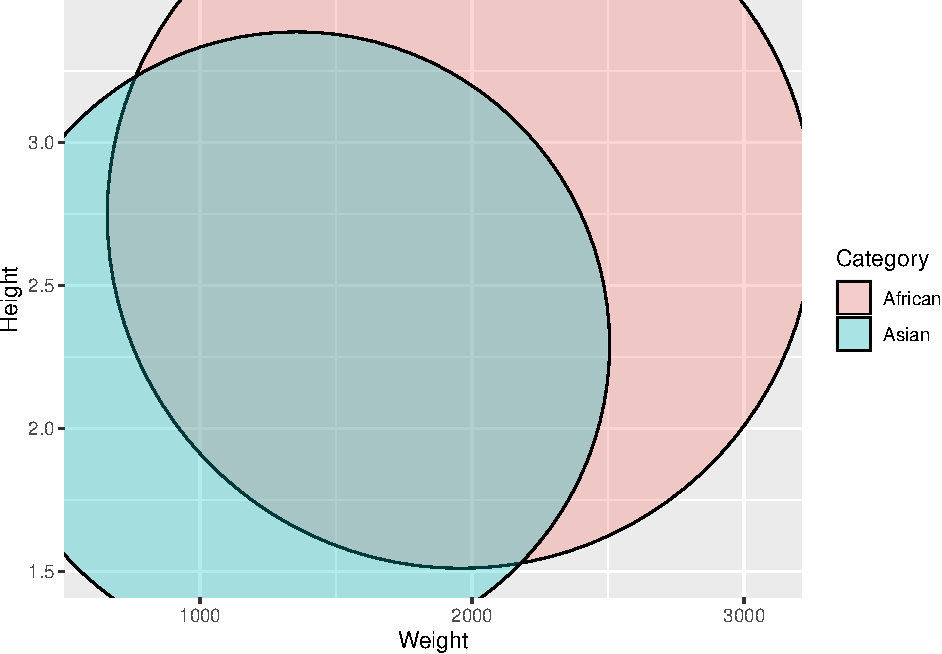
\includegraphics{Data-Visualisation-geom-Encyclopedia_files/figure-latex/unnamed-chunk-43-1.pdf}

With geom\_point

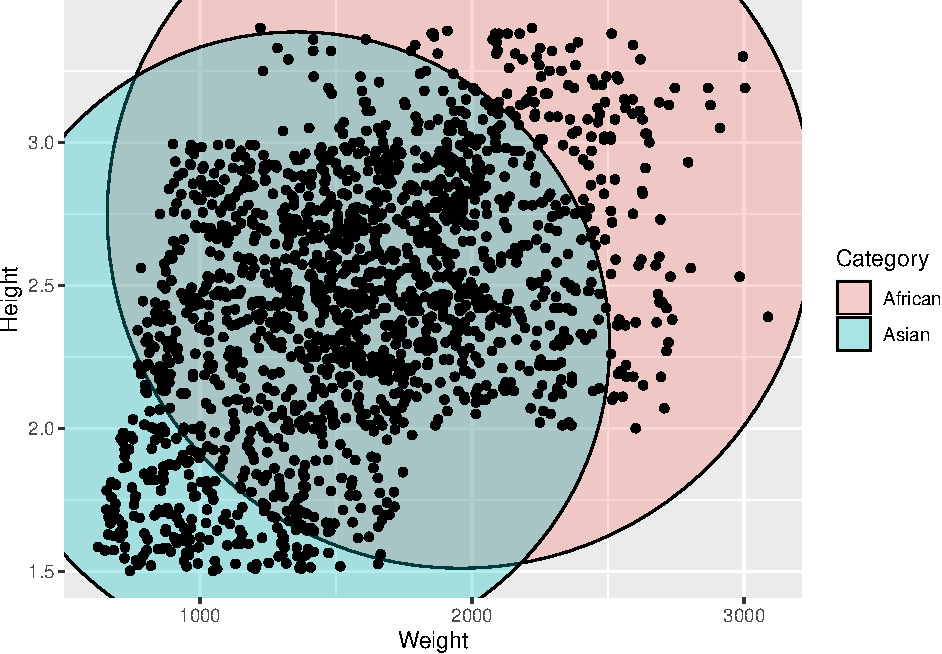
\includegraphics{Data-Visualisation-geom-Encyclopedia_files/figure-latex/unnamed-chunk-44-1.pdf}

\hypertarget{a-geom_axxxxx-4}{%
\chapter{A: geom\_axxxxx}\label{a-geom_axxxxx-4}}

\hypertarget{a-geom_axxxxx-5}{%
\chapter{A: geom\_axxxxx}\label{a-geom_axxxxx-5}}

\hypertarget{p-geom_p}{%
\chapter{P: geom\_p\ldots{}}\label{p-geom_p}}

\hypertarget{point}{%
\section{geom\_point}\label{point}}

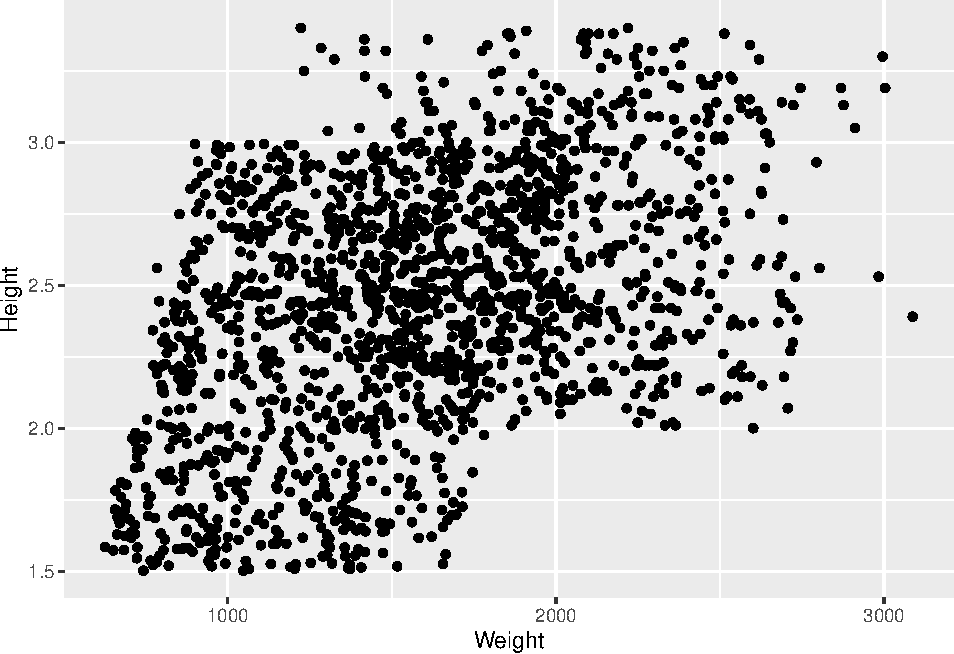
\includegraphics{Data-Visualisation-geom-Encyclopedia_files/figure-latex/unnamed-chunk-45-1.pdf}

\hypertarget{a-geom_axxxxx-6}{%
\chapter{A: geom\_axxxxx}\label{a-geom_axxxxx-6}}

\hypertarget{a-geom_axxxxx-7}{%
\chapter{A: geom\_axxxxx}\label{a-geom_axxxxx-7}}

\hypertarget{s-geom_s}{%
\chapter{S: geom\_s\ldots{}}\label{s-geom_s}}

\hypertarget{geom_signif}{%
\section{geom\_signif}\label{geom_signif}}

\begin{Shaded}
\begin{Highlighting}[]
\FunctionTok{ggplot}\NormalTok{(elephants, }\FunctionTok{aes}\NormalTok{(}\AttributeTok{y =}\NormalTok{ Weight, }\AttributeTok{x=}\NormalTok{Category)) }\SpecialCharTok{+} \FunctionTok{geom\_boxplot}\NormalTok{() }\SpecialCharTok{+}\NormalTok{ ggsignif}\SpecialCharTok{::}\FunctionTok{geom\_signif}\NormalTok{()}
\end{Highlighting}
\end{Shaded}

\begin{verbatim}
## Warning: Computation failed in `stat_signif()`
## Caused by error in `$<-.data.frame`:
## ! replacement has 1 row, data has 0
\end{verbatim}

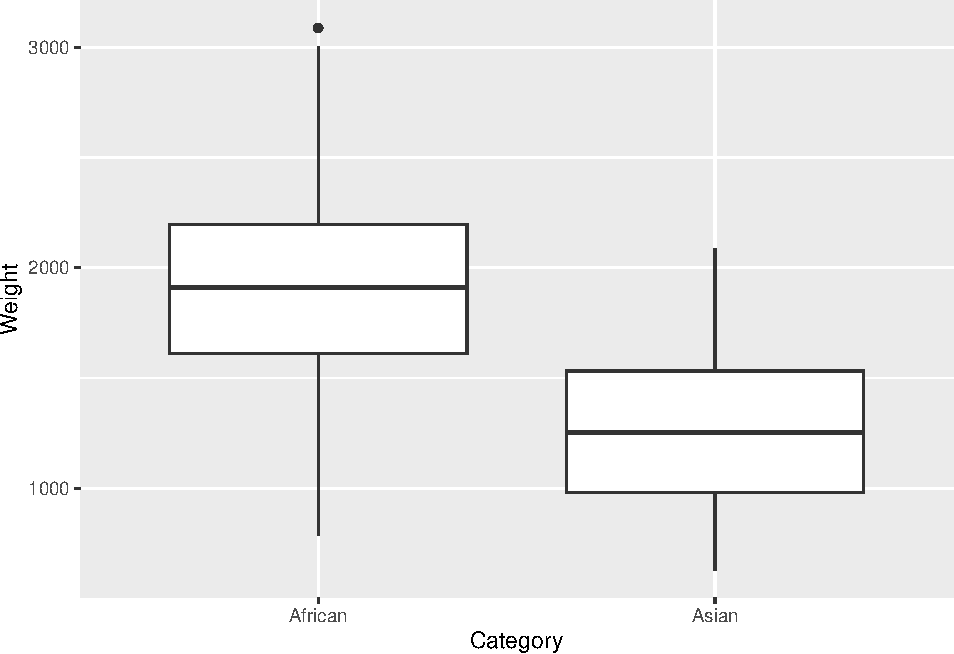
\includegraphics{Data-Visualisation-geom-Encyclopedia_files/figure-latex/unnamed-chunk-46-1.pdf}

\hypertarget{geom_smooth}{%
\section{geom\_smooth}\label{geom_smooth}}

\begin{verbatim}
## `geom_smooth()` using method = 'gam' and formula = 'y ~ s(x, bs = "cs")'
\end{verbatim}

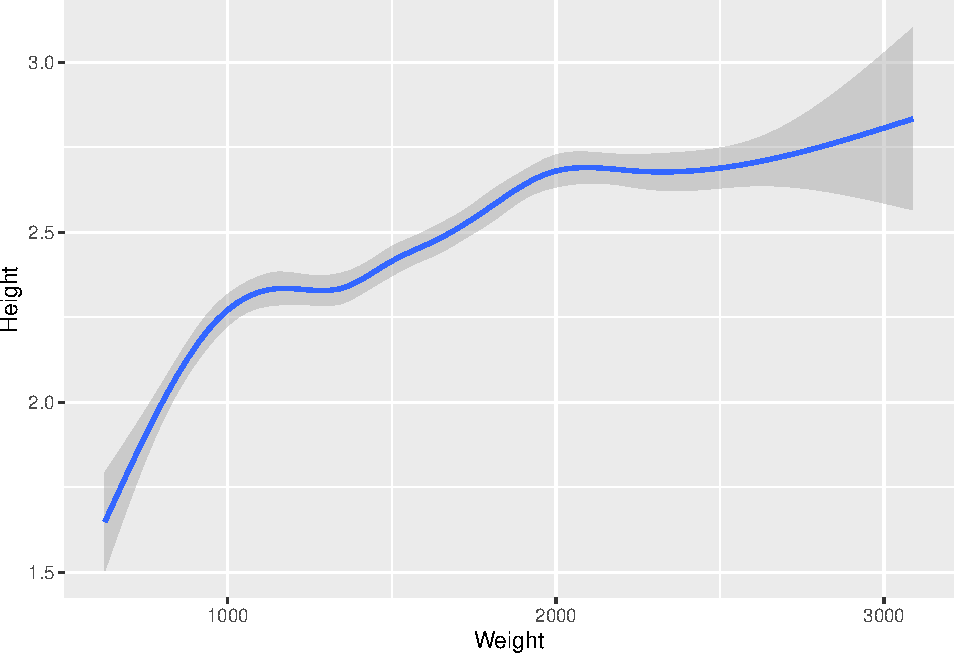
\includegraphics{Data-Visualisation-geom-Encyclopedia_files/figure-latex/unnamed-chunk-47-1.pdf}

\begin{verbatim}
## `geom_smooth()` using formula = 'y ~ x'
\end{verbatim}

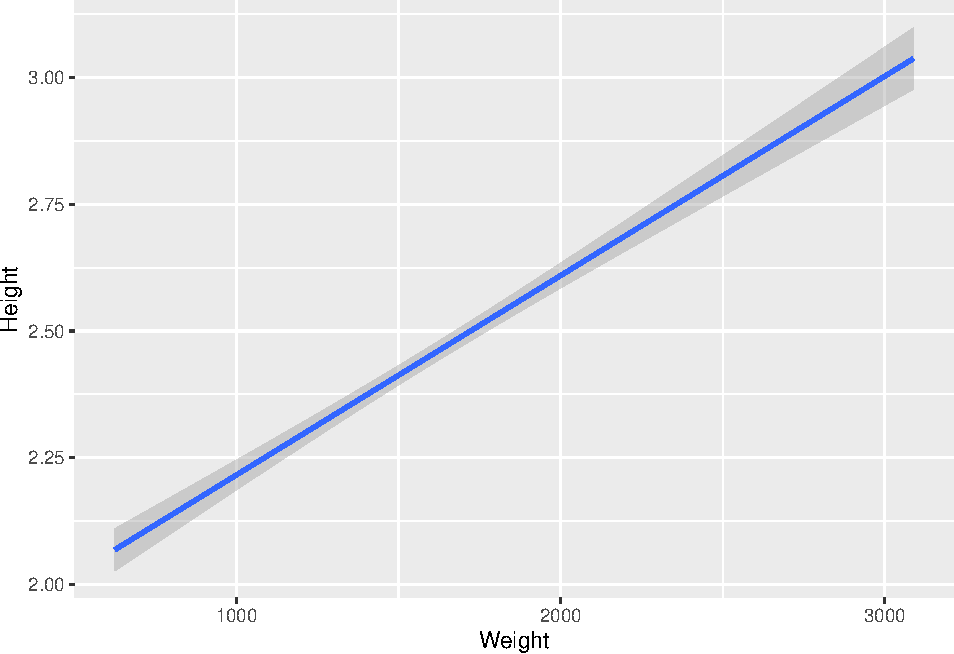
\includegraphics{Data-Visualisation-geom-Encyclopedia_files/figure-latex/unnamed-chunk-48-1.pdf}

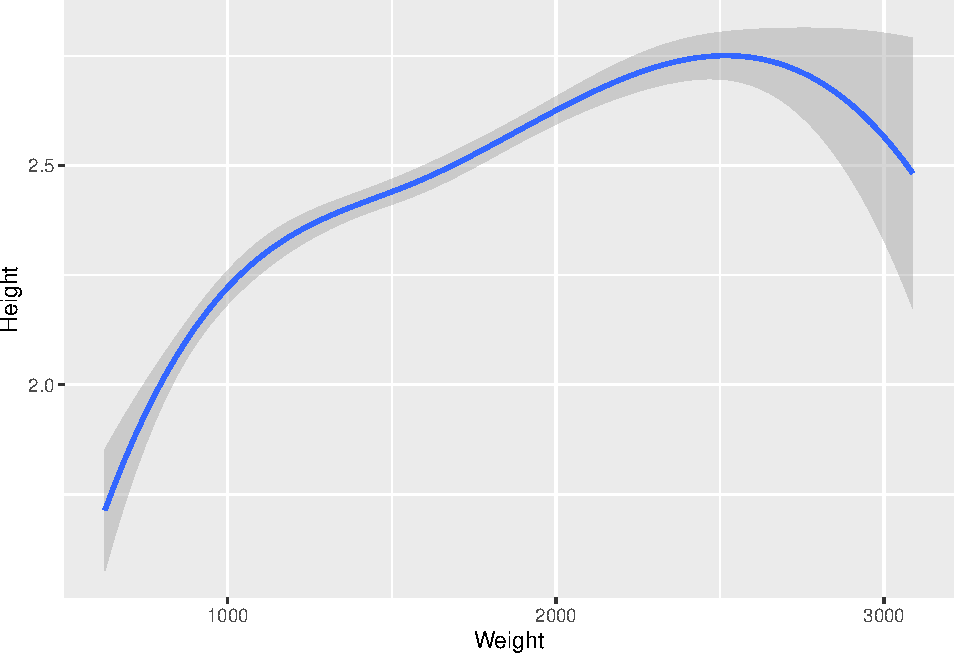
\includegraphics{Data-Visualisation-geom-Encyclopedia_files/figure-latex/unnamed-chunk-49-1.pdf}

\hypertarget{a-geom_axxxxx-8}{%
\chapter{A: geom\_axxxxx}\label{a-geom_axxxxx-8}}

\hypertarget{a-geom_axxxxx-9}{%
\chapter{A: geom\_axxxxx}\label{a-geom_axxxxx-9}}

\hypertarget{v-geom_v}{%
\chapter{V: geom\_v\ldots{}}\label{v-geom_v}}

\hypertarget{vline}{%
\section{geom\_vline}\label{vline}}

\textbf{Package: } ggplot2 \autocite{R-ggplot2}

\textbf{Book: }

\textbf{Description: } Draw a vertical line (\(X=c\)) for a given value of \(c\), which is known as \texttt{xintercept}.

\textbf{See also: } \protect\hyperlink{point}{geom\_point}, \protect\hyperlink{vline}{geom\_vline}, \protect\hyperlink{hline}{geom\_hline}

\textbf{Example:}

\begin{Shaded}
\begin{Highlighting}[]
\NormalTok{vline }\OtherTok{\textless{}{-}} \FunctionTok{ggplot}\NormalTok{(elephants.subset}\FloatTok{.100}\NormalTok{, }\FunctionTok{aes}\NormalTok{(}\AttributeTok{y =}\NormalTok{ Height, }\AttributeTok{x=}\NormalTok{Fore\_Feet\_Circumference)) }\SpecialCharTok{+} \FunctionTok{geom\_vline}\NormalTok{(}\AttributeTok{xintercept =} \FloatTok{1.25}\NormalTok{) }\SpecialCharTok{+} 
  \FunctionTok{labs}\NormalTok{(}\AttributeTok{title=}\StringTok{"A: \textasciigrave{}geom\_vline\textasciigrave{} only"}\NormalTok{) }\SpecialCharTok{+}
  \FunctionTok{theme}\NormalTok{(}\AttributeTok{aspect.ratio =} \DecValTok{1}\NormalTok{)}

\NormalTok{pointvline }\OtherTok{\textless{}{-}} \FunctionTok{ggplot}\NormalTok{(elephants.subset}\FloatTok{.100}\NormalTok{, }\FunctionTok{aes}\NormalTok{(}\AttributeTok{y =}\NormalTok{ Height, }\AttributeTok{x=}\NormalTok{Fore\_Feet\_Circumference)) }\SpecialCharTok{+} 
  \FunctionTok{geom\_point}\NormalTok{() }\SpecialCharTok{+} 
  \FunctionTok{geom\_vline}\NormalTok{(}\AttributeTok{xintercept =} \FloatTok{1.25}\NormalTok{) }\SpecialCharTok{+} 
  \FunctionTok{labs}\NormalTok{(}\AttributeTok{title=}\StringTok{"B: \textasciigrave{}geom\_point + geom\_vline\textasciigrave{} both"}\NormalTok{) }\SpecialCharTok{+}
  \FunctionTok{theme}\NormalTok{(}\AttributeTok{aspect.ratio =} \DecValTok{1}\NormalTok{)}

\FunctionTok{library}\NormalTok{(patchwork)}
\NormalTok{vline }\SpecialCharTok{|}\NormalTok{ pointvline}
\end{Highlighting}
\end{Shaded}

\begin{figure}
\centering
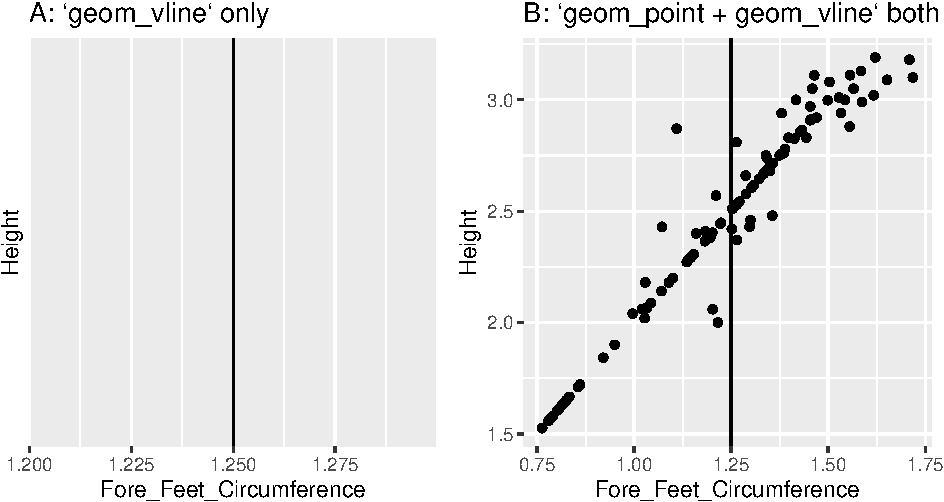
\includegraphics{Data-Visualisation-geom-Encyclopedia_files/figure-latex/unnamed-chunk-50-1.pdf}
\caption{\label{fig:unnamed-chunk-50}Illustration of (A) geom\_vline and (B) use of geom\_point and geom\_vline both}
\end{figure}

\hypertarget{geom_violin}{%
\section{geom\_violin}\label{geom_violin}}

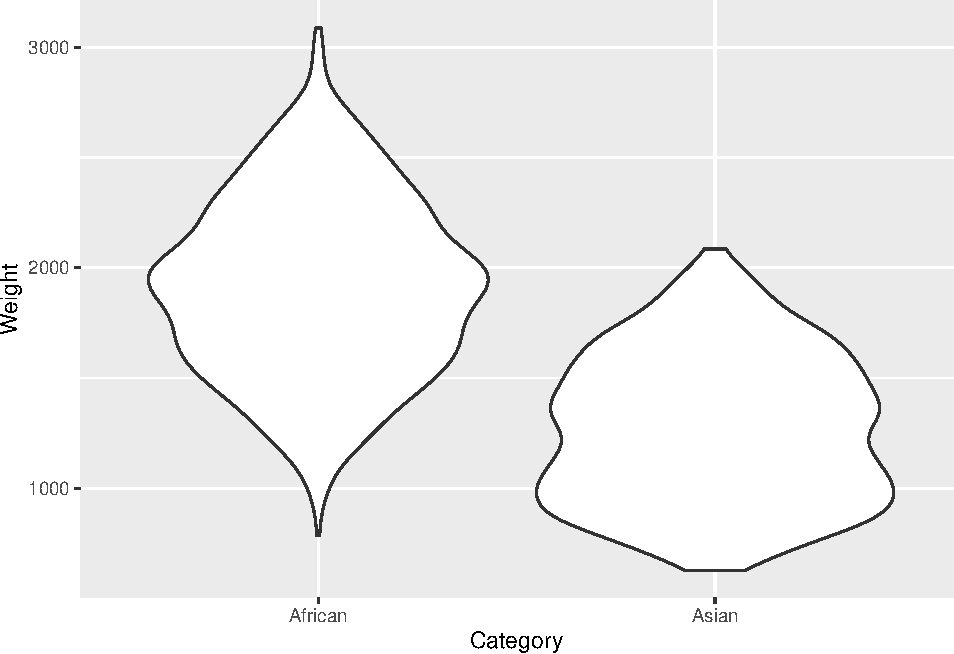
\includegraphics{Data-Visualisation-geom-Encyclopedia_files/figure-latex/unnamed-chunk-51-1.pdf}

Without trimming

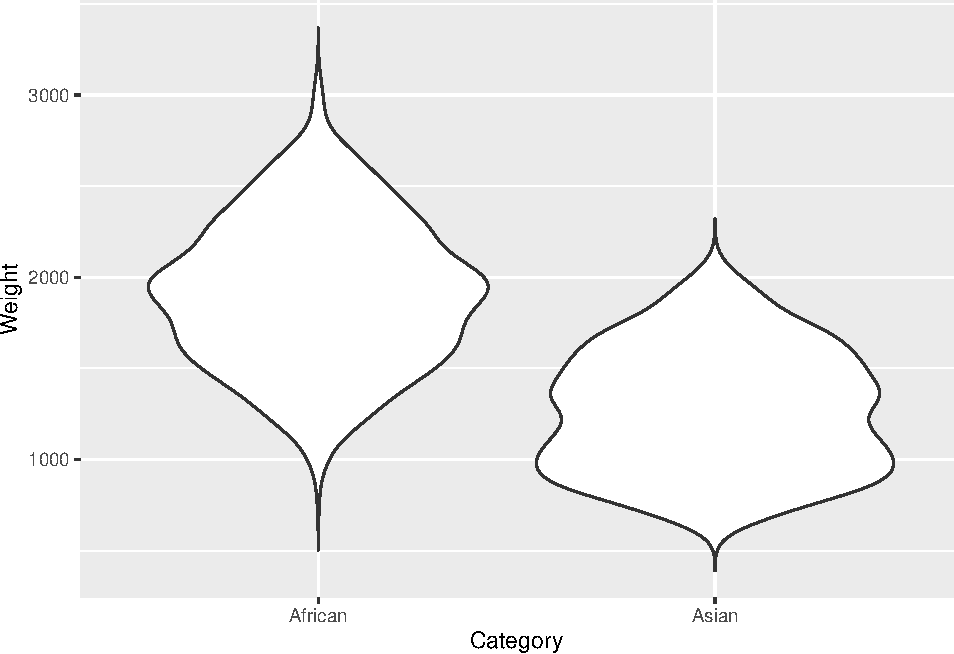
\includegraphics{Data-Visualisation-geom-Encyclopedia_files/figure-latex/unnamed-chunk-52-1.pdf}

Draw quantiles

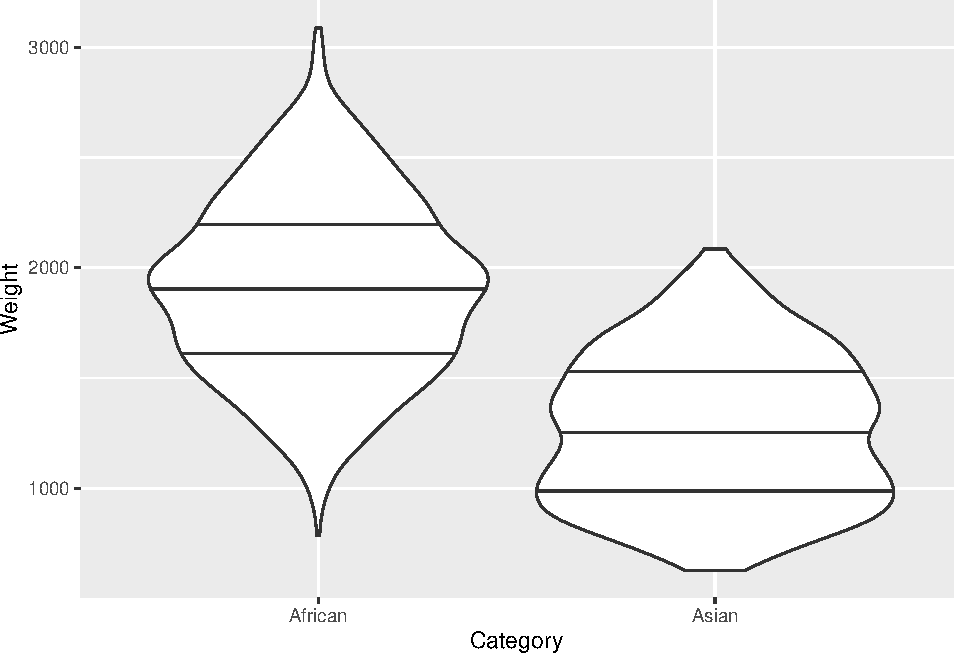
\includegraphics{Data-Visualisation-geom-Encyclopedia_files/figure-latex/unnamed-chunk-53-1.pdf}

\hypertarget{a-geom_axxxxx-10}{%
\chapter{A: geom\_axxxxx}\label{a-geom_axxxxx-10}}

\hypertarget{a-geom_axxxxx-11}{%
\chapter{A: geom\_axxxxx}\label{a-geom_axxxxx-11}}

\hypertarget{a-geom_axxxxx-12}{%
\chapter{A: geom\_axxxxx}\label{a-geom_axxxxx-12}}

\hypertarget{a-geom_axxxxx-13}{%
\chapter{A: geom\_axxxxx}\label{a-geom_axxxxx-13}}

\hypertarget{others}{%
\chapter{Others}\label{others}}

\hypertarget{ggpairs}{%
\section{ggpairs}\label{ggpairs}}

With all variables

\begin{Shaded}
\begin{Highlighting}[]
\NormalTok{GGally}\SpecialCharTok{::}\FunctionTok{ggpairs}\NormalTok{(elephants)}
\end{Highlighting}
\end{Shaded}

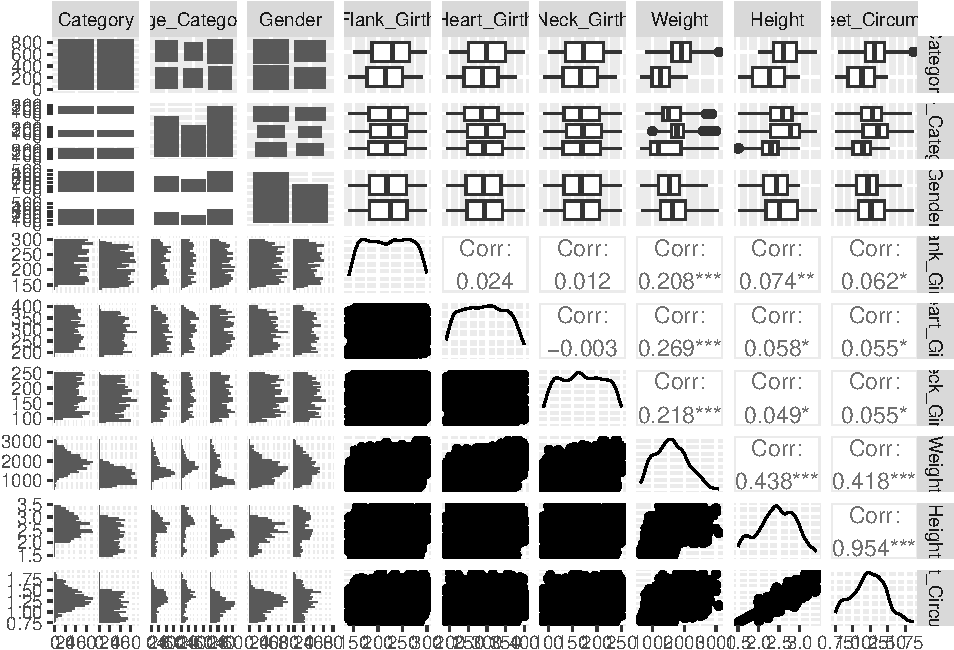
\includegraphics{Data-Visualisation-geom-Encyclopedia_files/figure-latex/unnamed-chunk-54-1.pdf}

With only numeric variables

\begin{Shaded}
\begin{Highlighting}[]
\NormalTok{elephants.numeric }\OtherTok{\textless{}{-}}\NormalTok{ elephants }\SpecialCharTok{|}\ErrorTok{\textgreater{}} \FunctionTok{select\_if}\NormalTok{(is.numeric)     }
\NormalTok{GGally}\SpecialCharTok{::}\FunctionTok{ggpairs}\NormalTok{(elephants.numeric)}
\end{Highlighting}
\end{Shaded}

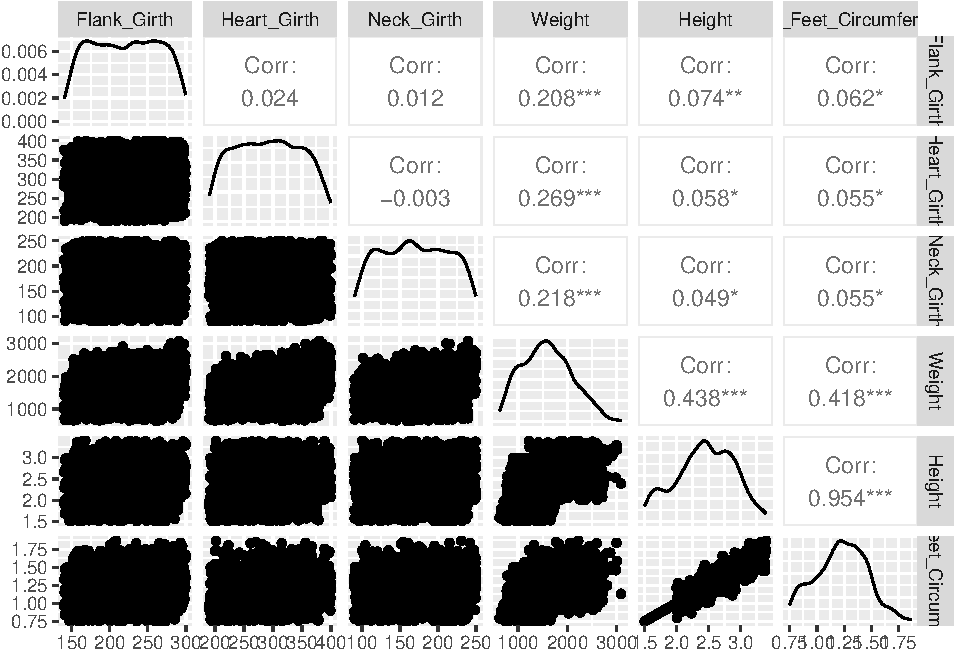
\includegraphics{Data-Visualisation-geom-Encyclopedia_files/figure-latex/unnamed-chunk-55-1.pdf}

Colour the points according to category

\begin{Shaded}
\begin{Highlighting}[]
\NormalTok{elephants.numeric }\OtherTok{\textless{}{-}}\NormalTok{ elephants }\SpecialCharTok{|}\ErrorTok{\textgreater{}} \FunctionTok{select\_if}\NormalTok{(is.numeric) }
\NormalTok{elephants.numeric}\SpecialCharTok{$}\NormalTok{Category }\OtherTok{\textless{}{-}}\NormalTok{ elephants}\SpecialCharTok{$}\NormalTok{Category}
\NormalTok{GGally}\SpecialCharTok{::}\FunctionTok{ggpairs}\NormalTok{(elephants.numeric, }\FunctionTok{aes}\NormalTok{(}\AttributeTok{col=}\NormalTok{Category))}
\end{Highlighting}
\end{Shaded}

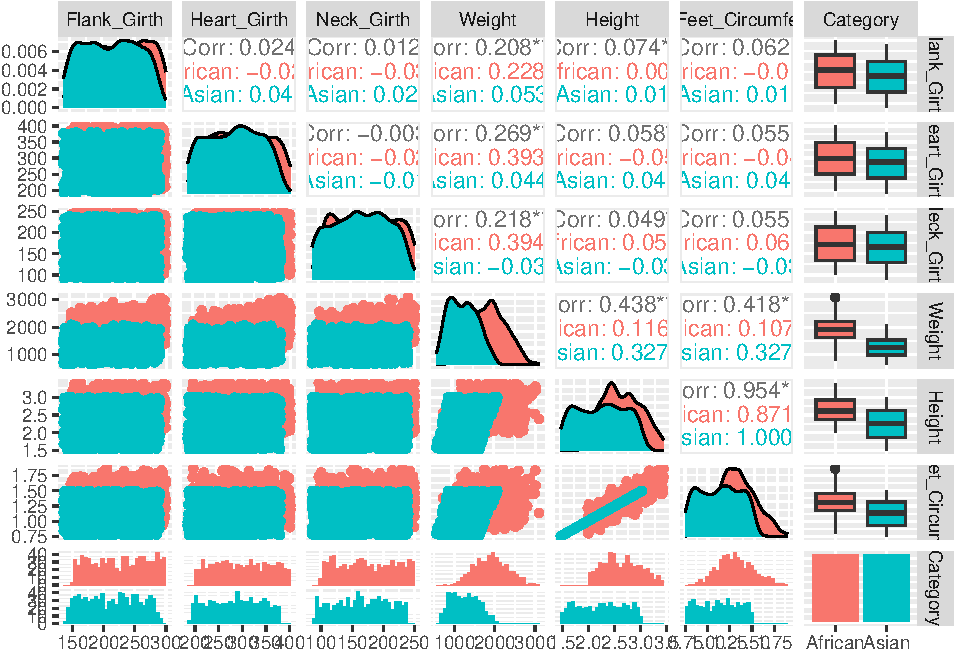
\includegraphics{Data-Visualisation-geom-Encyclopedia_files/figure-latex/unnamed-chunk-56-1.pdf}

\printbibliography

\end{document}
